% ======================================================================
% AAAI-27 submission format (converted from the ACL/ARR source).
% Structural/formatting changes only -- paper content is unchanged.
% The original ACL version is preserved in acl_latex.tex.
% ======================================================================

% ---- Required AAAI-27 preamble (per AuthorKit27; DO NOT CHANGE) --------
\documentclass[letterpaper]{article} % DO NOT CHANGE THIS
\usepackage[submission]{aaai2027}    % DO NOT CHANGE THIS (anonymous submission mode)
% The serif, sans-serif, and monospaced fonts are loaded automatically by
% aaai2027.sty (newtxtext, helvet, courier). Do NOT add times/helvet/courier
% or inconsolata -- they are forbidden and conflict with the style.
\usepackage[hyphens]{url}  % DO NOT CHANGE THIS
\usepackage{graphicx}      % DO NOT CHANGE THIS
\urlstyle{rm}              % DO NOT CHANGE THIS
\def\UrlFont{\rm}          % DO NOT CHANGE THIS
\usepackage{natbib}        % DO NOT CHANGE THIS (aaai2027 sets the .bst automatically)
\usepackage{caption}       % DO NOT CHANGE THIS
\frenchspacing             % DO NOT CHANGE THIS
% Keep section numbers on (2 = sections + subsections) so the paper's many
% \ref{sec:...}/\ref{apx:...} cross-references resolve. AAAI permits 0/1/2;
% never exceed 2 (subsubsection numbering breaks the style).
\setcounter{secnumdepth}{2}
\pdfinfo{
/TemplateVersion (2027.1)
}

% ---- Packages carried over from the ACL source (content-neutral) ------
\usepackage[T1]{fontenc}
\usepackage[utf8]{inputenc}
\usepackage{microtype}
\usepackage{amsmath}
\usepackage{mathtools}
\usepackage{amssymb}
\usepackage{algorithm}   % AAAI-recommended for algorithms
\usepackage{algorithmic} % AAAI-recommended for algorithms
% bbm is hard-blocked by aaai2027.sty (Type-3 fonts). Use dsfont (Type-1) and
% alias \mathbbm so any \mathbbm{...} in the source still renders identically.
\usepackage{dsfont}
\newcommand{\mathbbm}[1]{\mathds{#1}}
\usepackage{booktabs}
\usepackage[most]{tcolorbox}
\usepackage{multirow}
\usepackage{subcaption}
\usepackage{xcolor}
\definecolor{AlgGreen}{RGB}{34,139,34}

% ---- Robust asset paths (compile-root-independent) --------------------
% Figures and \input files are under latex/. These search paths let the
% document compile whether the working directory is the repo root or latex/
% (Overleaf vs. local), so nothing silently drops. \includegraphics and
% \input below are given WITHOUT the "latex/" prefix and resolved here.
\graphicspath{{latex/figs/}{figs/}}
\makeatletter
\def\input@path{{latex/}{./}}
\makeatother

% ---- Custom macros carried over verbatim from the ACL source ----------
% Comment macro for algorithm right-margin annotations
\newcommand{\algcmt}[1]{\hfill \textcolor{AlgGreen}{\ensuremath{\triangleright}\,#1}}

% Author annotation macros (disable/remove before submission)
\newcommand{\ml}[1]{\textcolor{orange}{\bf [lan: #1]}}
\newcommand{\mh}[1]{\textcolor{teal}{\bf [Hunter: #1]}}
\newcommand{\al}[1]{\textcolor{blue}{\bf [Alex: #1]}}

% Compact standard-deviation suffix for table cells: $0.314\std{0.016}$.
\newcommand{\std}[1]{{\scriptstyle\,\pm #1}}

\newtcolorbox{promptbox}[1]{
  colback=gray!10,
  colframe=gray!70!black,
  title=#1,
  fonttitle=\bfseries,
  arc=3mm,
  boxrule=0.8pt,
  left=6pt,
  right=6pt,
  top=6pt,
  bottom=6pt
}

\newtcolorbox{answerbox}[1]{
  colback=blue!5,
  colframe=blue!80!black,
  title=#1,
  fonttitle=\bfseries,
  arc=3mm,
  boxrule=1pt,
  left=6pt,
  right=6pt,
  top=6pt,
  bottom=6pt
}

% Qualitative counterfactual example box (appendix).
% title is braced so commas inside the title don't get parsed as pgfkeys.
\newtcolorbox{examplebox}[2][]{
  colback=gray!4,
  colframe=gray!50!black,
  title={#2},
  fonttitle=\bfseries,
  arc=2mm,
  boxrule=0.6pt,
  left=6pt,
  right=6pt,
  top=6pt,
  bottom=6pt,
  breakable,
  #1
}

% If the title and author information does not fit in the area allocated, uncomment the following
%
%\setlength\titlebox{<dim>}
%
% and set <dim> to something 5cm or larger.

% ---- Cross-reference bridge to the main paper (resolves \ref to main-paper
% ---- tables/figures/sections). Requires aaai_main.aux to exist: compile the
% ---- main paper once, then this file. xr does not embed links (hyperref-free).
\usepackage{xr}
\externaldocument{aaai_main}

\title{Supplementary Material\\Gumbel Machine: Counterfactual Student Writing Generation via Gumbel Noise Steering}
\author{
    Anonymous Submission
}
\affiliations{
    %
}

\begin{document}
\maketitle

\appendix

\section{Appendix}\label{sec:appendix}

%% =====================================================================
%% TEXT SECTIONS
%% =====================================================================

\subsection{Per-Criterion Results} \label{apx:tradeoffs}

\begin{table*}[!htbp]
\centering
% \small
\setlength{\tabcolsep}{3pt}
\scalebox{.85}{
\begin{tabular}{ll  cc  cc  cc  cc  cc}
\toprule
\textbf{Model} & \textbf{Approach}
  & $\text{Sim}^\uparrow$ & $\text{Val}^\uparrow$
  & $\text{Sim}^\uparrow$ & $\text{Val}^\uparrow$
  & $\text{Sim}^\uparrow$ & $\text{Val}^\uparrow$
  & $\text{Sim}^\uparrow$ & $\text{Val}^\uparrow$
  & $\text{Sim}^\uparrow$ & $\text{Val}^\uparrow$ \\
\midrule
\multicolumn{2}{l}{\textit{CLASSE}}
  & \multicolumn{2}{c}{\textbf{Main Idea}}
  & \multicolumn{2}{c}{\textbf{Details}}
  & \multicolumn{2}{c}{\textbf{Organization}}
  & \multicolumn{2}{c}{\textbf{Wording}}
  & \multicolumn{2}{c}{\textbf{Language}} \\
\midrule
\multirow{3}{*}{Haiku}
  & ME       & 0.285 & 0.064 & 0.282 & 0.243 & 0.279 & 0.015 & 0.266 & 0.341 & 0.289 & 0.056 \\
  & ICL      & 0.274 & $\textbf{0.365}$ & 0.268 & 0.454 & 0.279 & 0.158 & 0.292 & $\textbf{0.513}$ & 0.294 & 0.072 \\
  & I\&R     & $\textbf{0.482}$ & 0.263 & $\textbf{0.402}$ & $\textbf{0.651}$ & $\textbf{0.501}$ & $\textbf{0.177}$ & $\textbf{0.407}$ & 0.486 & $\textbf{0.461}$ & $\textbf{0.365}$ \\
\cmidrule(l){2-12}
\multirow{3}{*}{Sonnet}
  & ME       & 0.450 & 0.139 & 0.344 & 0.599 & 0.348 & 0.114 & 0.362 & 0.651 & 0.377 & 0.216 \\
  & ICL      & 0.377 & $\textbf{0.577}$ & 0.320 & 0.711 & 0.362 & $\textbf{0.496}$ & 0.380 & $\textbf{0.804}$ & 0.356 & $\textbf{0.432}$ \\
  & I\&R     & $\textbf{0.646}$ & 0.410 & $\textbf{0.520}$ & $\textbf{0.766}$ & $\textbf{0.562}$ & 0.201 & $\textbf{0.524}$ & 0.419 & $\textbf{0.516}$ & 0.373 \\
\cmidrule(l){2-12}
\multirow{4}{*}{Llama}
  & ME       & 0.305 & 0.165 & 0.315 & 0.224 & 0.299 & 0.265 & 0.341 & 0.154 & 0.310 & 0.107 \\
  & ICL      & 0.288 & 0.272 & 0.308 & 0.381 & 0.305 & 0.516 & 0.320 & 0.182 & 0.320 & 0.282 \\
  & I\&R     & $\textbf{0.528}$ & 0.117 & $\textbf{0.440}$ & 0.096 & $\textbf{0.529}$ & 0.112 & $\textbf{0.498}$ & 0.092 & $\textbf{0.494}$ & 0.099 \\
  % & BH       & $\textbf{0.546}$ & 0.171 & $\textbf{0.557}$ & 0.145 & $\textbf{0.554}$ & 0.165 & $\textbf{0.596}$ & 0.152 & $\textbf{0.548}$ & 0.206 \\
  & GM (Ours) & 0.364 & $\textbf{0.820}$ & 0.334 & $\textbf{0.780}$ & 0.387 & $\textbf{0.769}$ & 0.412 & $\textbf{0.666}$ & 0.458 & $\textbf{0.306}$ \\
\cmidrule(l){2-12}
\multirow{4}{*}{Qwen}
  & ME       & $\textbf{0.648}$ & 0.163 & $\textbf{0.667}$ & 0.247 & 0.579 & 0.239 & 0.558 & 0.281 & 0.432 & 0.230 \\
  & ICL      & 0.349 & 0.190 & 0.347 & 0.248 & 0.359 & 0.156 & $\textbf{0.620}$ & 0.217 & 0.326 & 0.137 \\
  & I\&R     & 0.524 & 0.282 & 0.403 & 0.540 & 0.474 & 0.328 & 0.388 & $\textbf{0.385}$ & 0.450 & 0.286 \\
  % & BH       & $\textbf{0.693}$ & 0.140 & $\textbf{0.702}$ & 0.236 & 0.619 & 0.244 & 0.585 & 0.252 & 0.468 & 0.235 \\
  & GM (Ours) & 0.506 & $\textbf{0.729}$ & 0.455 & $\textbf{0.761}$ & $\textbf{0.624}$ & $\textbf{0.483}$ & 0.615 & 0.312 & $\textbf{0.677}$ & $\textbf{0.544}$ \\
\midrule
\multicolumn{2}{l}{\textit{DREsS}}
  & \multicolumn{2}{c}{\textbf{Content}}
  & \multicolumn{2}{c}{\textbf{Language}}
  & \multicolumn{2}{c}{\textbf{Organization}}
  & \multicolumn{4}{c}{} \\
\midrule
\multirow{3}{*}{Haiku}
  & ME       & 0.308 & 0.105 & 0.337 & 0.123 & 0.292 & 0.052 & & & & \\
  & ICL      & 0.307 & 0.170 & 0.328 & 0.097 & 0.307 & 0.109 & & & & \\
  & I\&R     & $\textbf{0.340}$ & $\textbf{0.566}$ & $\textbf{0.460}$ & $\textbf{0.216}$ & $\textbf{0.352}$ & $\textbf{0.541}$ & & & & \\
\cmidrule(l){2-12}
\multirow{3}{*}{Sonnet}
  & ME       & 0.332 & 0.544 & 0.431 & $\textbf{0.411}$ & 0.363 & 0.363 & & & & \\
  & ICL      & 0.372 & $\textbf{0.556}$ & 0.502 & 0.386 & 0.380 & 0.509 & & & & \\
  & I\&R     & $\textbf{0.438}$ & 0.435 & $\textbf{0.571}$ & 0.212 & $\textbf{0.426}$ & $\textbf{0.566}$ & & & & \\
\cmidrule(l){2-12}
\multirow{4}{*}{Llama}
  & ME       & 0.312 & 0.323 & 0.307 & 0.143 & 0.295 & 0.097 & & & & \\
  & ICL      & 0.357 & 0.327 & 0.320 & 0.239 & 0.312 & 0.227 & & & & \\
  & I\&R     & 0.296 & $\textbf{0.489}$ & 0.322 & 0.116 & 0.307 & 0.370 & & & & \\
  % & BH       & 0.448 & 0.220 & 0.405 & 0.136 & $\textbf{0.353}$ & 0.087 \\
  & GM (Ours) & $\textbf{0.637}$ & 0.307 & $\textbf{0.498}$ & $\textbf{0.371}$ & $\textbf{0.344}$ & $\textbf{0.507}$ & & & & \\
\cmidrule(l){2-12}
\multirow{4}{*}{Qwen}
  & ME       & 0.298 & 0.266 & 0.305 & 0.195 & 0.287 & 0.128 & & & & \\
  & ICL      & 0.301 & 0.235 & 0.388 & 0.104 & 0.324 & 0.100 & & & & \\
  & I\&R     & 0.248 & $\textbf{0.718}$ & 0.337 & $\textbf{0.312}$ & 0.351 & $\textbf{0.582}$ & & & & \\
  % & BH       & 0.299 & 0.297 & 0.308 & 0.166 & 0.294 & 0.159 \\
  & GM (Ours) & $\textbf{0.511}$ & 0.414 & $\textbf{0.604}$ & 0.200 & $\textbf{0.707}$ & 0.248 & & & & \\
\bottomrule
\end{tabular}}
\caption{Per-criterion breakdown comparing counterfactual approaches (ME - Minimal-Edit, ICL - In-Context Learning, I\&R - Identify-and-Replace, GM - Gumbel Machine) on Similarity and Validity on the CLASSE (top) and DREsS (bottom) datasets. Bold marks the best value per model within each (criterion, metric) cell. }
\label{tab:appendix_per_criterion}
\end{table*}
We report a per-criterion expansion of the aggregate similarity and validity measurements reported for Llama-3 and Qwen3 in 
Table~\ref{tab:appendix_per_criterion}. We observe that the within-model similarity-validity ordering is consistent across criteria for both open-weight backbones where GM tends to maximize validity with minimal tradeoff for similarity. The clearest exception is the CLASSE ``Wording'' criterion, where ICL on Qwen achieves the highest similarity, suggesting that Qwen has exceptional paraphrase capabilities when provided in-context demonstrations.

\subsection{Instruction Prompts} \label{apx:prompts}

We include the details of the instructions passed to the various open-weight models during counterfactual generation. The base counterfactual prompt is shown both including the reference summary (Figure~\ref{apx:prompt_ref}) and excluding it (Figure~\ref{fig:exc_prompt}) for two distinct criteria. The Identify-and-Replace (I\&R) prompt is shown in Figure~\ref{fig:ir_prompt}, illustrated on the DREsS ``Language'' criterion. Format is identical for other criteria with rubric details replaced.

\subsection{Tuning Gumbel Noise Control} \label{apx:tuning}

In Figure~\ref{fig:pareto-front}, we report the results of our experiments to tune the controllable $\beta$ parameter in the GM. In these experiments, we vary the control signal across a range of values for GM and compare with Vocab Bias, a simple decoding strategy that adds a tunable $\alpha$ to all logits for all tokens in the reference summary \cite{yang_fudge_2021}. For GM, we sweep the control parameter $\beta$ across the values $\beta \in \{0.001, 0.1, 0.2, 0.3, 0.4, 1.0\}$ for CLASSE and $\beta \in \{0.05, 0.2, 0.4, 0,5, 0.6, 0.7, 0.8, 1.0\}$ for DREsS. Higher values of $\beta$ emphasize similarity to the original student response, while lower values prioritize satisfying the desired target score. For Vocab Bias, we sweep the control parameter $\alpha$ across the values $\alpha \in \{0.01, 5.0, 10.0\}$ for CLASSE and $\alpha \in \{0.01, 1.0, 5.0\}$ for DREsS. Higher values of $\alpha$ induce stronger similarity to reference tokens. We observe that values outside these ranges result in collapses in model fluency due to excessive logit manipulation.

Comparing the two approaches, we observe that for GM, increasing values of $\beta$ enable a trade-off between similarity that can explore a much wider range of the Pareto front compared to Vocab Bias. Further, we observe that GM tends to maintain higher validity with increasing similarity values. These observations suggest that recovered Gumbel noise provides a more effective control signal for generating similar counterfactual randomness than using token-level heuristics for similarity control. This finding suggests that similarity control in LLMs is more robust when the entire sampling trajectory and random states are considered rather than solely token-level alignment.

\subsection{Scoring Model} \label{apx:scoring}

\begin{figure}
        \centering
        \begin{subfigure}{\linewidth}
            \centering
            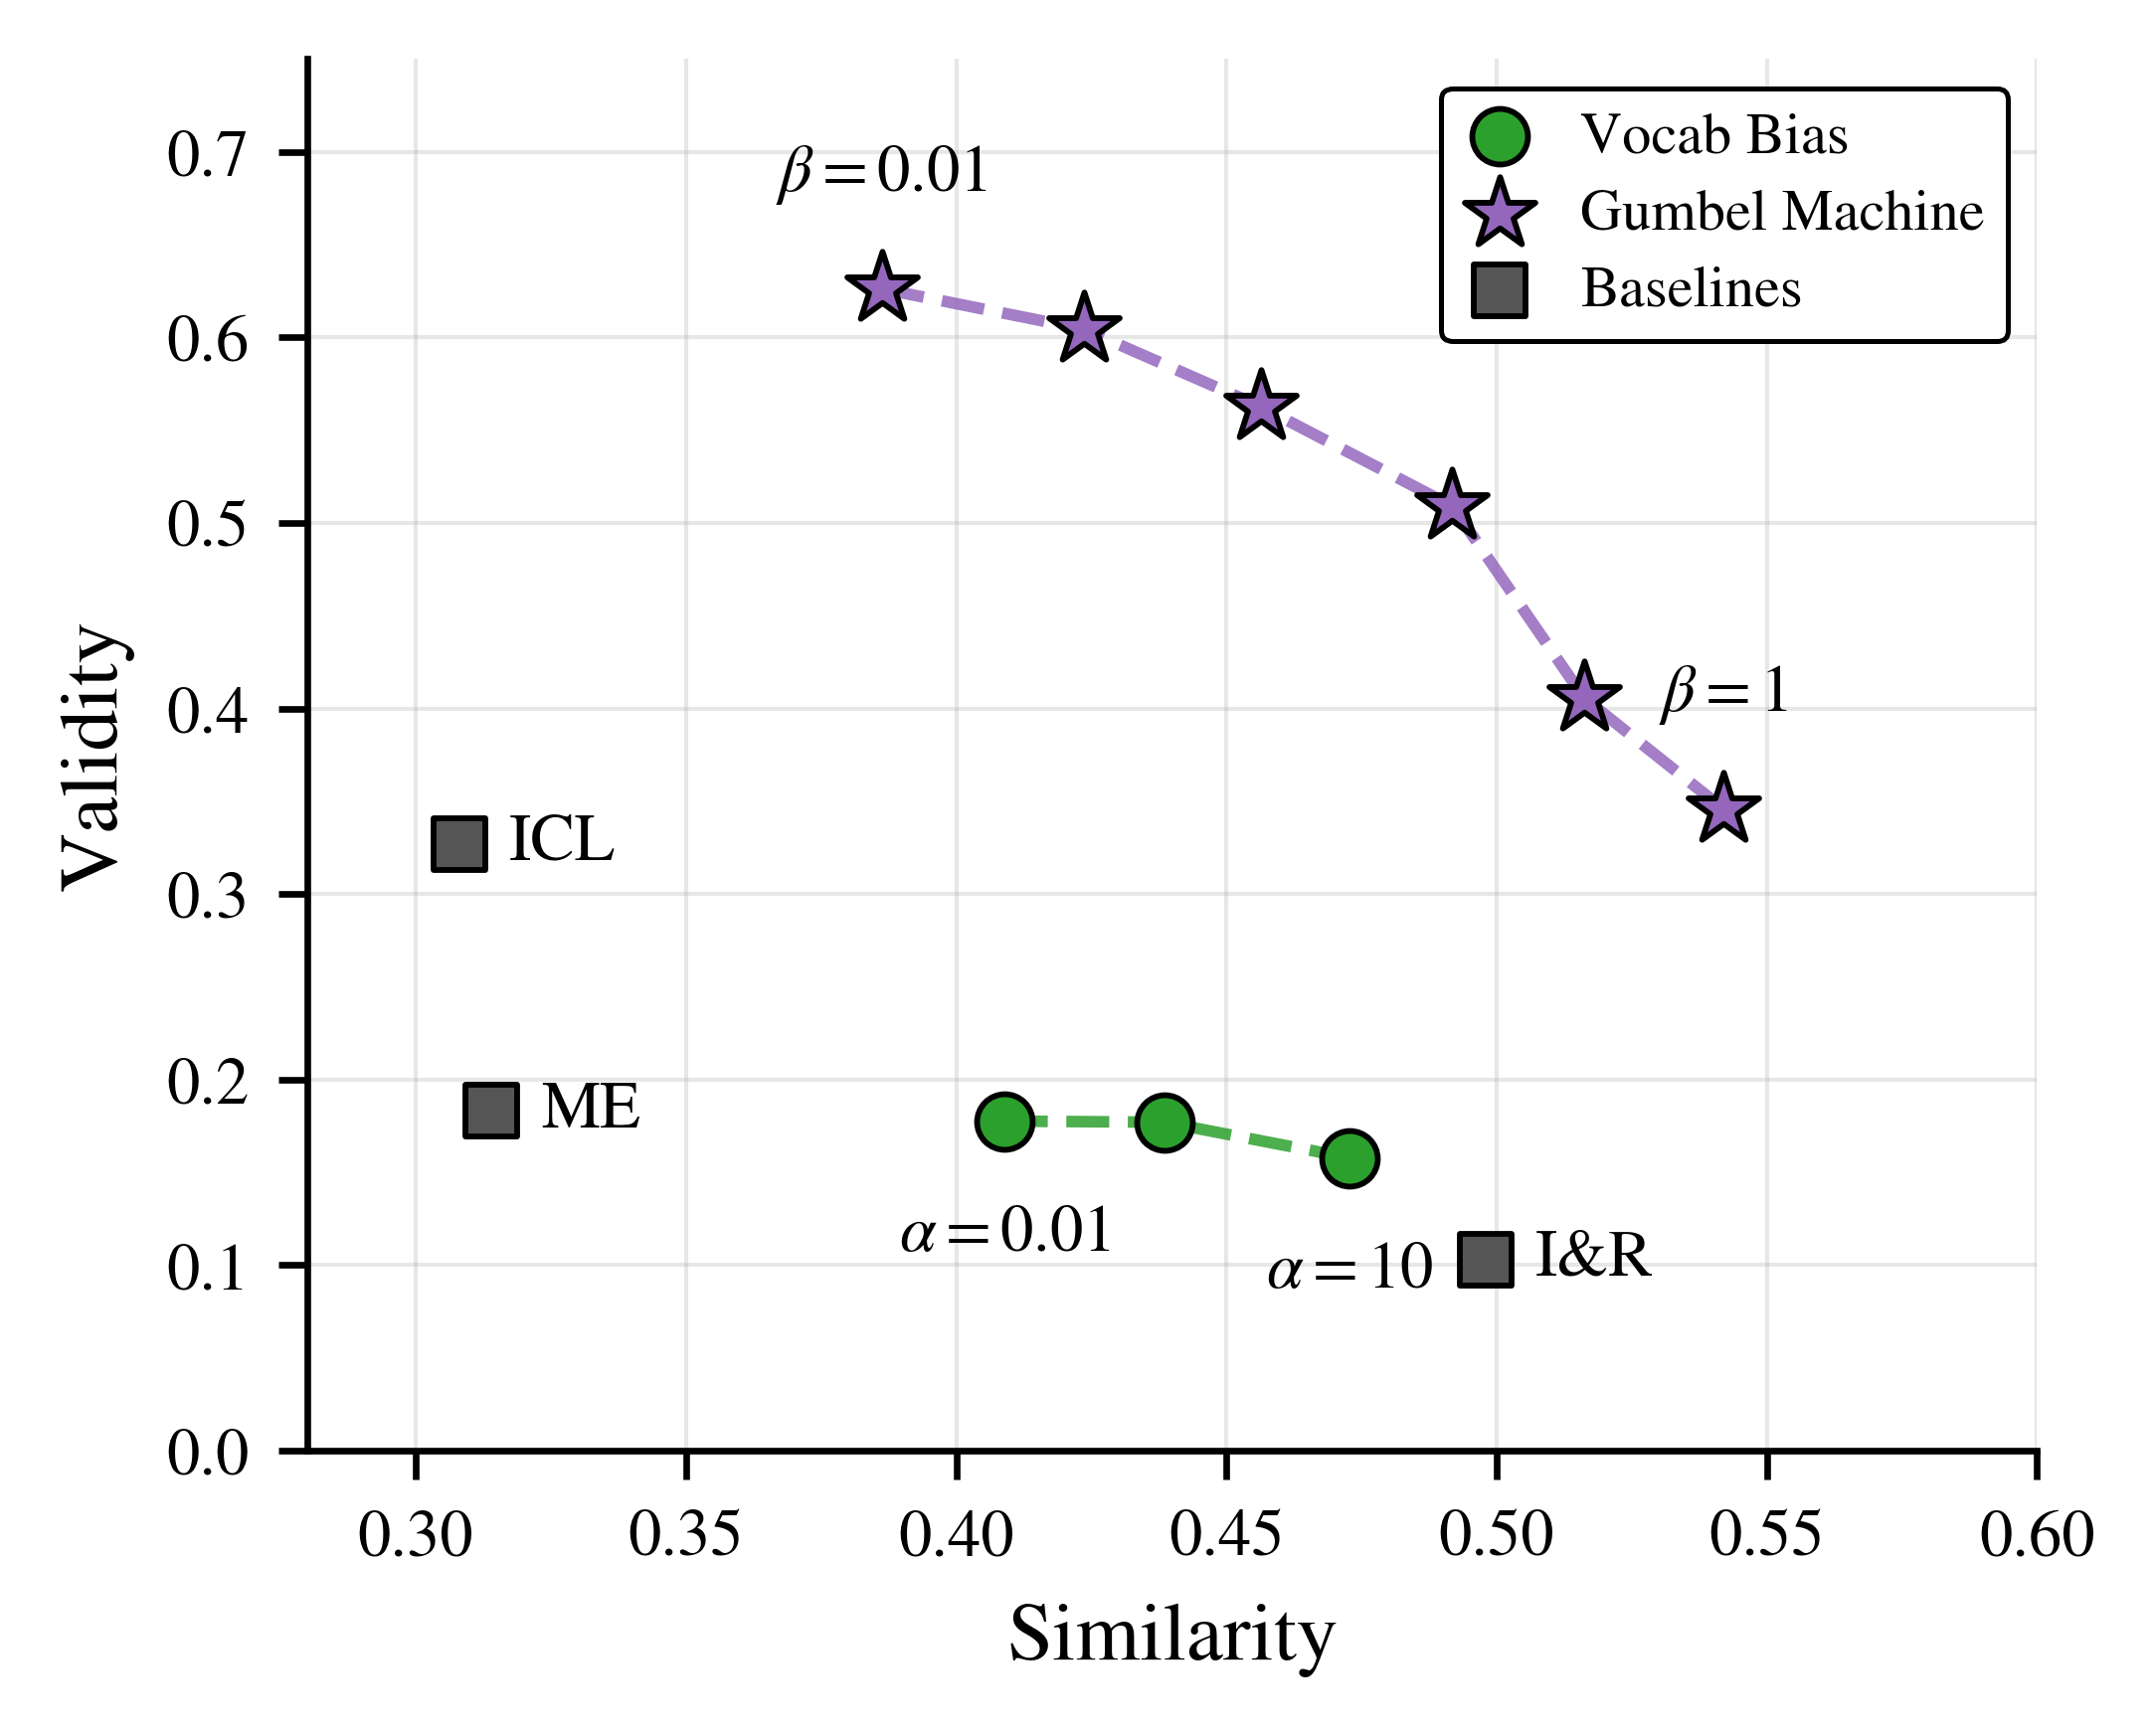
\includegraphics[width=\linewidth]{paper_tradeoff_v4_larger.png}
            \caption{CLASSE}
            \label{fig:pareto-front-classe}
        \end{subfigure}

        \vspace{0.6em}

        \begin{subfigure}{\linewidth}
            \centering
            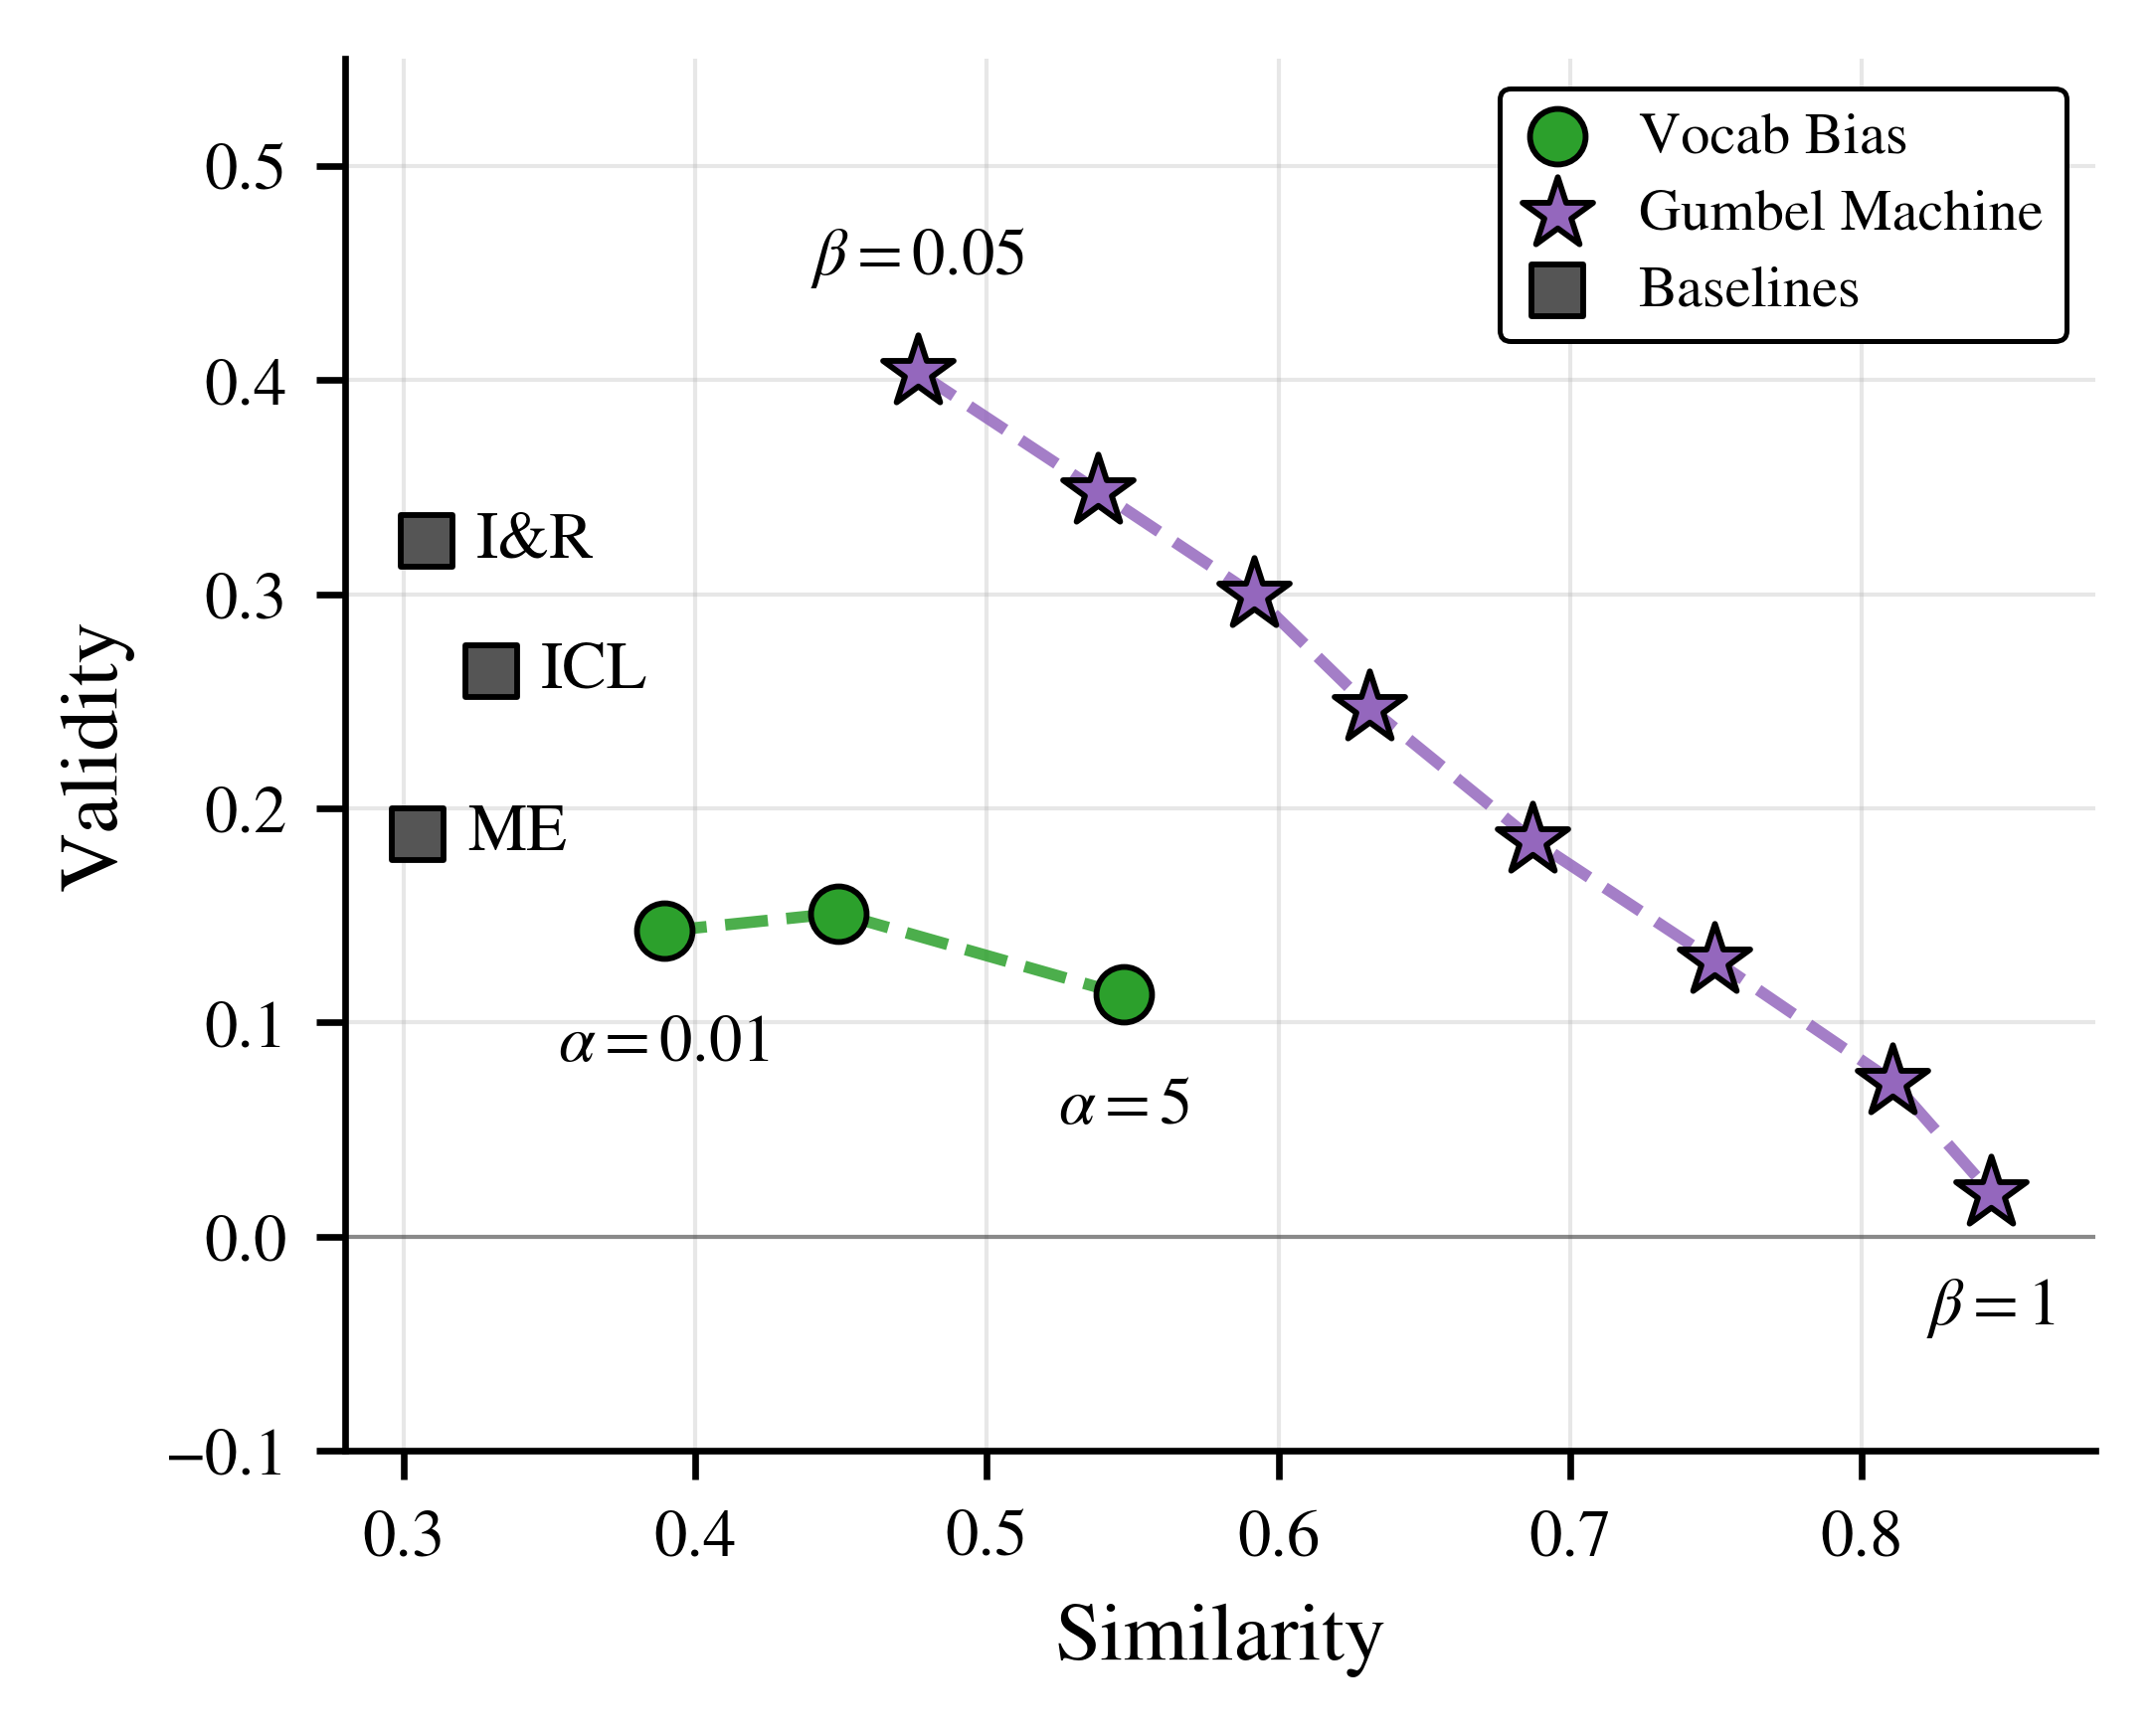
\includegraphics[width=\linewidth]{dress_tradeoff_v1_larger.png}
            \caption{DREsS}
            \label{fig:pareto-front-dress}
        \end{subfigure}
        \caption{Similarity–validity trade-offs comparing Gumbel Machine with a logit bias and baseline approaches (ME - Minimal-Edit, ICL - In-Context Learning, I\&R - Identify-and-Replace) on CLASSE (top) and DREsS (bottom). Gumbel Machine provides a tunable tradeoff between competing metrics, occupying a different region of the Pareto frontier than the logit-bias baseline.}
        \label{fig:pareto-front}
\end{figure}

\begin{table*}[h]
\centering
\small
\setlength{\tabcolsep}{6pt}
\scalebox{.9}{
\begin{tabular}{ll  c  ccc}
\toprule
& & \textbf{BERT} & \multicolumn{3}{c}{\textbf{GPT-4.1 family}} \\
\cmidrule(lr){3-3} \cmidrule(lr){4-6}
\textbf{Dataset} & \textbf{Criterion} & \texttt{ModernBERT}-base & \texttt{GPT-4.1} (prompted) & \texttt{GPT-4.1-mini} (prompted) & \texttt{GPT-4.1-mini} (fine-tuned) \\
\midrule
\multirow{6}{*}{CLASSE}
  & Main Idea     & 0.566 & 0.632 & 0.590 & \textbf{0.683} \\
  & Details       & 0.616 & 0.473 & 0.476 & \textbf{0.690} \\
  & Organization  & 0.607 & 0.495 & 0.393 & \textbf{0.628} \\
  & Wording       & 0.542 & 0.463 & 0.366 & \textbf{0.522} \\
  & Language      & 0.423 & 0.543 & 0.497 & \textbf{0.598} \\
  & \textbf{Mean} & 0.551 & 0.521 & 0.464 & \textbf{0.624} \\
\midrule
\multirow{4}{*}{DREsS}
  & Content      & 0.540 & 0.211 & 0.289 & \textbf{0.652} \\
  & Organization & 0.490 & 0.278 & 0.213 & \textbf{0.598} \\
  & Language     & 0.475 & 0.208 & 0.252 & \textbf{0.553} \\
  & \textbf{Mean} & 0.502 & 0.232 & 0.251 & \textbf{0.601} \\
\bottomrule
\end{tabular}}
\caption{Per-criterion QWK agreement between scoring models and human raters on the CLASSE and DREsS validation sets.}
\label{apx:scoring_per_criterion}
\end{table*}

Figure~\ref{fig:score_prompt} shows the instructions passed to our scoring model for the ``Language'' criterion. Rubric details are modified relative to each criterion. The model is prompted with top $p=1.0$ and temperature $0$ to reduce randomness, with an instruction to provide justification before scoring to encourage Chain-of-Thought reasoning.

\paragraph{Scoring Model Comparison} Our final scoring model is a fine-tuned \texttt{GPT-4.1-mini} model, trained per criterion. We report scoring-model comparisons across four configurations: (i) a fine-tuned BERT encoder following \cite{fernandez_automated_2022}, (ii) prompting the larger \texttt{GPT-4.1} model, (iii) prompting \texttt{GPT-4.1-mini}, and (iv) fine-tuned \texttt{GPT-4.1-mini}. Table~\ref{apx:scoring_per_criterion} reports per-criterion QWK against human ratings on a held-out validation set for CLASSE and DREsS, respectively. Across both datasets the fine-tuned \texttt{GPT-4.1-mini} achieves the highest mean QWK (CLASSE $0.624$, DREsS $0.601$) and outperforms every other scoring configuration on nearly every criterion.

For the BERT scoring model, we fine-tune a \texttt{ModernBERT-base} encoder with a linear regression head over the integer rubric scores using mean-squared-error loss. For both prompted and fine-tuned GPT models we use the template shown in Figure~\ref{fig:score_prompt}, sampled with temperature $0$ and top-$p=1.0$. For fine-tuning, we use OpenAI's hosted fine-tuning API on \texttt{gpt-4.1-mini-2025-04-14}, training one checkpoint per criterion on the criterion-specific train split with the same prompt template used at inference.

\subsection{Prompt Ablation} \label{apx:prompt-ablate}

\begin{table}[t]
\centering
\small
\begin{tabular}{lcc}
\toprule
\textbf{Criterion} & \textbf{Reference} & \textbf{No Reference} \\
\midrule
Main Idea  & 0.626 & 0.347 \\
Details    & 0.604 & 0.315 \\
Cohesion   & 0.597 & 0.315 \\
Wording    & 0.611 & 0.352 \\
Language   & 0.622 & 0.325 \\
\midrule
\textbf{Overall} & 0.612 & 0.331 \\
\bottomrule
\end{tabular}
\caption{Ablation study on reference conditioning influence on recovered Gumbel noise control effectiveness. Table reports average similarity scores across counterfactuals. Across all criteria, reference hinting shows higher effectiveness of the recovered noise.}
\label{tab:foresight_ablation}
\end{table}

In Table~\ref{tab:foresight_ablation}, we report results of an ablation study where we compare how inclusion and exclusion of the reference summary in the prompt influence the effectiveness of $\beta$-Hindsight control. In this ablation, we include/exclude the reference both during noise recovery and replay, set $\beta=1.0$, and run hindsight sampling on the base Llama-3 setting. We see an average counterfactual similarity score of $0.331$ when excluding the reference, which is similar to ME. However, when including the reference at recovery, the generated counterfactual summary is much more similar to the reference. These results suggest a nuanced interaction between the replayed Gumbel noise and the conditioning context, highlighting the importance of reference inclusion for effective $\beta$-Hindsight control. One possible explanation is that, when the reference tokens are highly certain (logit value of the reference token significantly exceeds that of other ones), the recovered noise is not strong enough to significantly alter the LLM's overall output trajectory, and only provides small adjustments at a given timestep. On the contrary, when the reference tokens are less certain, the recovered noise encodes nuanced information, resulting in a volatile control signal with conflicting objectives that can significantly alter the output trajectory. 
% We leave further investigation into the mechanics of effective controllable Gumbel noise recovery as an interesting direction for future work.

\subsection{Dataset Details} \label{apx:classe}

We report detailed descriptions for each CLASSE criterion in Table~\ref{apx:criteria} and Table~\ref{apx:rubric} details score definitions for each possible value. Figure~\ref{fig:token_counts} provides a breakdown of the summary and passage lengths in the dataset. Summaries are approximately 68 words in length and passages are approximately 297 words (calculated by simple space separation). We report detailed descriptions for each DREsS criterion in Table~\ref{apx:dress_criteria} and Table~\ref{apx:dress_rubric} details score definitions for each possible value. Figure~\ref{fig:dress_token_counts} provides a breakdown of the essay and writing-prompt lengths in the dataset. Essays are approximately 310 words in length and writing prompts are approximately 30 words.

\subsection{Training Details} \label{apx:training}

We train all GM checkpoints using parameter-efficient fine-tuning on \texttt{LLaMA-3.1-8B-Instruct} and \texttt{Qwen3-4B-Instruct-2507}. The pipeline runs supervised fine-tuning (SFT) on counterfactual prompt-target pairs, followed by direct preference optimization (DPO) on score-gap preference pairs constructed from the same training split. For both stages, we train a rank-$32$ LoRA adapter with dropout $0.05$ for all attention and MLP projections using an AdamW optimizer. For SFT, we use a constant learning rate of $5\!\times\!10^{-5}$ with weight decay $0.01$, and in DPO we use a cosine schedule at $2\!\times\!10^{-5}$ against the frozen SFT LoRA as the reference policy.

We estimate our experiments to spend 350 NVIDIA GPU-hours across A100, L40, A40, and RTX 8000 GPUs. In addition to closed-weight API access to Claude Haiku 4.5, Claude Sonnet 4.6, and 8 fine-tuned GPT-4.1-mini judges.

% \paragraph{Preference pair construction.} DPO pairs are bucketed per dataset. For DREsS, we group essays by (writing prompt, target-criterion score) and require the score gap on the target criterion to be at least $2.0$; we additionally constrain the rejected essay's two non-target criteria to stay within $\pm 1.0$ of the chosen essay so the preference signal reflects only the target criterion. We sample one rejected essay per (chosen essay, alternative score) bucket, yielding approximately $800$ training and $133$ validation pairs per criterion. For CLASSE, we group by source passage and accept all non-zero score gaps with no non-target filter, since CLASSE's five interrelated criteria leave few candidates under a strict non-target constraint; this yields approximately $10{,}000$--$11{,}000$ training pairs per criterion.

\subsection{Human Evaluation Details} \label{sec:apdx-human-eval}

% \paragraph{Recruitment and demographics.} The five evaluators were recruited via Upwork \cite{upwork} with explicit screening for documented K--12 or post-secondary English teaching experience. All evaluators reported at least eight years of English teaching experience, with several reporting twenty-five or more years, spanning middle school, high school, and university settings in the United States. Each evaluator completed an IRB-approved consent process before participating; the task took approximately two hours and evaluators were compensated \$60.

\paragraph{Task structure.} Each evaluator was shown 50 (passage, student summary, rewrite A, rewrite B) tuples on the CLASSE dataset, stratified across the five criteria and across the original student score on the target criterion. The pair of rewrites was sampled one from GM and one from the Minimal-Edit baseline at matched automated validity (target score $4$); ordering was randomized and the generating approach was hidden from the evaluator. For each tuple, evaluators answered three per-rewrite questions independently for A and B on a 1--3 scale (None / Slight / Clear), and then three direct-comparison questions with options $\{A, B, \text{Same}\}$. The task took evaluators roughly 2 hours, and we paid them \$60 each, which is significantly higher than the minimum wage in the country where this study was conducted. All evaluators gave consent before participating via an IRB-approved consent form.

\paragraph{Calibration material.} Evaluators were provided with a reference document, available throughout the task, that contained: (i) a description of the rewrite-comparison task and a worked positive/negative rewrite example; (ii) detailed guidance on each of the six questions with concrete anchors for the 1--3 scale; (iii) a sample passage paired with each rubric criterion; and (iv) for each criterion, the score-level rubric (1--4) together with an example student summary at every rubric score for calibration. Table~\ref{apx:rubric} and Table~\ref{apx:criteria} provide detailed definitions shown to evaluators for each criterion.

\paragraph{Interface.} Figures~\ref{fig:label_interface_1} and~\ref{fig:label_interface_2} show the evaluation interface used in the study. The interface presents the passage and the student summary alongside the two rewrites, with the per-rewrite questions appearing first (Figure~\ref{fig:label_interface_1}) and the direct-comparison questions appearing second (Figure~\ref{fig:label_interface_2}).

\paragraph{Inter-rater Agreement} We observe an inter-rater agreement (Krippendorff's $\alpha$) on the similarity rating Likert of $\alpha=0.29$ across all four raters, increasing to $\alpha=0.43$ when restricted to the three raters who actively differentiated on this dimension (one rater frequently selected "Same" on similarity comparisons, 36/50 tasks). The directional finding that GM produces more similar rewrites is replicated by all four raters individually.

% \paragraph{Sample.} The headline analysis is computed over $150$ ratings from three contributing evaluators on $50$ stratified $(\text{passage}, \text{summary}, \text{rewrite~A}, \text{rewrite~B})$ tuples, balanced as $10$ tuples per CLASSE criterion and stratified across the original student score on the target criterion. The pair of rewrites for each tuple was sampled with one rewrite from GM and one from the Minimal-Edit baseline at matched automated validity (target score~$4$).

% \paragraph{Per-criterion preferences.} Table~\ref{tab:eval_per_criterion} reports the per-criterion GM win rate on the three pairwise questions (ties excluded). Aggregated across criteria, the headline pattern is that GM is preferred on similarity (63\% GM wins, $p\!=\!0.024$) and roughly tied on improvement and feedback. The criterion-level breakdown reveals that this aggregate hides substantial criterion-specific variation: GM is preferred on every dimension for the Language and Details criteria, while it loses on Main Idea and on the criterion-targeted comparison for Organization (Cohesion), where evaluators preferred the Minimal-Edit rewrites despite GM's clear similarity advantage on the same criterion (88\% GM win on the similarity comparison).

% \paragraph{Preferences scale with student score.} The student's original score on the target criterion (always less than the target of $4$) appears to modulate GM's similarity advantage. Table~\ref{tab:eval_per_ref} bins ratings by the student's reference score; the GM win rate on the ``more similar'' comparison rises sharply from $48\%$ at reference~$1$ to $92\%$ at reference~$3$ (binomial $p\!<\!10^{-3}$), and a Spearman rank correlation between the reference score and the GM-minus-ME Likert difference on the per-rewrite similarity item gives $\rho = 0.279$ ($p = 0.0004$, $n = 150$). The criterion preferences also drift in the same direction, with GM moving from a slight loss at reference~$1$ to a slight win at reference~$3$, though neither end is individually significant. This pattern is consistent with GM being most useful when the student writing is already close to the target rubric score, leaving room for minimal-edit-style improvement.

% \paragraph{Similarity preference predicts overall preference.} Conditioning on the same evaluator's response to the ``more similar'' comparison reveals a strong interaction between the similarity judgment and the other two pairwise picks. When the evaluator marks GM as more similar to the student writing, GM is preferred on improvement in $65\%$ of those cases and on feedback in $68\%$; when the evaluator marks Minimal-Edit as more similar, GM's win rate on improvement drops to $39\%$ and on feedback to $38\%$. The full $3\!\times\!3$ contingency table is significant for both the improvement comparison ($\chi^2(4) = 14.8$, $p = 5.2\!\times\!10^{-3}$) and the feedback comparison ($\chi^2(4) = 23.4$, $p = 1.1\!\times\!10^{-4}$). This is consistent with the main-text claim that evaluators who recognize the similarity advantage of GM also prefer it pedagogically.


% \paragraph{Inter-rater agreement.} Cohen's $\kappa$ on the pairwise comparisons across the three rater pairs (averaged) is $0.03$ for ``better on criterion,'' $0.16$ for ``more similar,'' and $-0.02$ for ``better feedback''; quadratic-weighted $\kappa$ on the per-rewrite Likert items is $0.15$--$0.27$. These values are at the lower end of typical human-evaluation reliability and reflect the difficulty of grading subtle differences between two rewrites that already share matched automated validity. \ml{agreement is really low. looks bad}
% Despite the low pairwise agreement on individual tuples, the per-rater marginal preferences (Table~\ref{tab:eval_per_rater}) are directionally consistent across the three evaluators, with all three favoring GM on similarity and clustering around chance for improvement and feedback. We therefore interpret the headline findings as aggregate preference patterns rather than reliable per-task judgments.

%% =====================================================================
%% QUALITATIVE EXAMPLES
%% =====================================================================

\onecolumn
\subsection{Qualitative Counterfactual Examples} \label{apx:qualitative}

\begin{examplebox}[label=ex:civil-service]{Example 1 --- Civil Service}
\textbf{Student writing} (Score 3):

\begin{quote}\itshape
Civil service jobs are available for all people.\,\, These jobs have fair pay from the merit system.\,\, These jobs are filled by the top applicants.\,\, This process is time consuming, but he benefits to having a civil service job out ways the steps that need to be taken.
\end{quote}

\textbf{GM rewrite} (sim $0.50$):

\begin{quote}\itshape
Civil service jobs are available for all people, offering a wide range of positions from clerks to law enforcement. These jobs are filled by the top applicants through the merit system, which ensures fair pay and fair treatment for all employees. The merit system is set up to protect the employee and provide equal and fair pay. This process is time consuming, but the benefits of having a civil service job outweigh the steps that need to be taken.
\end{quote}

\textbf{ME rewrite} (sim $0.30$):

\begin{quote}\itshape
Civil service jobs offer opportunities to men and women at various levels of government, including city, county, state, and federal. The merit system is used to recruit the most qualified individuals for each position, ensuring fair pay, training, and treatment regardless of background. With a range of job types available, from administrative roles to law enforcement and skilled trades, civil service offers secure employment options for those willing to invest the time and effort required to secure a position.
\end{quote}
\end{examplebox}
\captionof{figure}{Example of a counterfactual rewrite where Gumbel Machine (GM) remains similar in precise wording and structure to the student writing while inserting relevant intermediate sentences and clauses to improve the summary. Minimal Edit (ME) instead reorganizes the content significantly and does not preserve the student's original wording.}
\label{ex:civil-service}


\clearpage

\begin{examplebox}{Example 2 --- Global Warming}
\textbf{Student writing} (Score 1):

\begin{quote}\itshape
Most people in California are more environmentally conscious than in other places in the country. They also don't believe that the government is doing enough to stop this.
\end{quote}

\textbf{GM rewrite} (sim $0.24$):

\begin{quote}\itshape
Most Californians are very concerned about global warming. They believe that the earth is warming too much and that it will affect living things on the earth. A survey was taken in California to see how people felt about global warming. The results showed that most people in California are very concerned about global warming and want the state to work on the problem. They are not happy with the federal government's handling of the issue and want the state to start working on it immediately.
\end{quote}

\textbf{ME rewrite} (sim $0.19$):

\begin{quote}\itshape
California residents are particularly concerned about the state of the planet, linking the issue to global warming. They believe that this warming poses a threat to living things. Californians want the state to take responsibility for investigating the problem.

Californians are deeply disturbed when it comes to the federal government's response to global warming. This year, they are more worried than ever, feeling the problem is getting worse. They want the state to take action immediately.

Californians want the state to start working on the problem as soon as possible, rather than waiting for the federal government to act.
\end{quote}
\end{examplebox}


\clearpage

\begin{examplebox}{Example 3 --- Ecological Pyramids}
\textbf{Student writing} (Score 3):

\begin{quote}\itshape
Ecologists construct a pyramid of numbers based on the population sizes of organisms in each trophic level. Sometimes population sizes decrease at each higher trophic level. This is not always true. For example, one tree can be food for 50,000 insects. In this case, the pyramid would be inverted.

Energy decreases at each succeeding trophic level. The total energy transfer from one trophic level to the next is only about ten percent because organisms fail to capture and eat all the food available at the trophic level below them. When an organism consumes food, it uses some of the energy in the food for metabolism, some for building body tissues, and some is given off as waste.
\end{quote}

\textbf{GM rewrite} (sim $0.75$):

\begin{quote}\itshape
Ecologists construct a pyramid of numbers based on the population sizes of organisms in each trophic level. Sometimes population sizes decrease at each higher trophic level. This is not always true. For example, one tree can be food for 50,000 insects. In this case, the pyramid would be inverted. Energy decreases at each succeeding trophic level. The total energy transfer from one trophic level to the next is only about ten percent because organisms fail to capture and eat all the food available at the trophic level below them. When an organism consumes food, it uses some of the energy in the food for metabolism, some for building body tissues, and some is given off as waste. When the organism is eaten, the energy that was used to build body tissue is available as energy to be used by the organism that consumed it. The energy lost at each successive trophic level enters the environment as heat.
\end{quote}

\textbf{ME rewrite} (sim $0.34$):

\begin{quote}\itshape
Ecologists use ecological pyramids to model the distribution of matter and energy within an ecosystem. This type of pyramid shows how energy flows through an ecosystem. The initial source of energy for all ecological pyramids is energy from the sun, which decreases at each succeeding trophic level due to inefficient energy transfer. The total energy transfer from one trophic level to the next is only about ten percent. When an organism consumes food, it uses some of the energy in the food for metabolism, some for building body tissues, and some is given off as waste, with the energy lost at each successive trophic level entering the environment as heat. Ecologists also construct pyramids of numbers based on population sizes, which sometimes decrease at each higher trophic level, but can also be inverted, such as when one tree is food for 50,000 insects.
\end{quote}
\end{examplebox}

\twocolumn

%% =====================================================================
%% NUMERICAL TABLES
%% =====================================================================

% \begin{table*}[h]
% \centering
% \setlength{\tabcolsep}{3pt}
% \begin{tabular}{ll  cc  cc  cc  cc  cc}
% \toprule
% & & \multicolumn{2}{c}{\textbf{Main Idea}}
% & \multicolumn{2}{c}{\textbf{Details}}
% & \multicolumn{2}{c}{\textbf{Organization}}
% & \multicolumn{2}{c}{\textbf{Wording}}
% & \multicolumn{2}{c}{\textbf{Language}} \\
% \cmidrule(lr){3-4} \cmidrule(lr){5-6} \cmidrule(lr){7-8} \cmidrule(lr){9-10} \cmidrule(lr){11-12}
% \multirow{-2}{*}{\textbf{Model}} & \multirow{-2}{*}{\textbf{Method}}
%   & $\text{Sim}^\uparrow$ & $\text{Val}^\uparrow$
%   & $\text{Sim}^\uparrow$ & $\text{Val}^\uparrow$
%   & $\text{Sim}^\uparrow$ & $\text{Val}^\uparrow$
%   & $\text{Sim}^\uparrow$ & $\text{Val}^\uparrow$
%   & $\text{Sim}^\uparrow$ & $\text{Val}^\uparrow$ \\
% \midrule
% \multirow{5}{*}{Llama}
%   & ME       & 0.305 & 0.165 & 0.315 & 0.224 & 0.299 & 0.265 & 0.341 & 0.154 & 0.310 & 0.107 \\
%   & ICL      & 0.288 & 0.272 & 0.308 & 0.381 & 0.305 & 0.516 & 0.320 & 0.182 & 0.320 & 0.282 \\
%   & I\&R     & 0.528 & 0.117 & 0.440 & 0.096 & 0.529 & 0.112 & 0.498 & 0.092 & 0.494 & 0.099 \\
%   % & BH       & $\textbf{0.546}$ & 0.171 & $\textbf{0.557}$ & 0.145 & $\textbf{0.554}$ & 0.165 & $\textbf{0.596}$ & 0.152 & $\textbf{0.548}$ & 0.206 \\
%   & GM (Ours) & 0.364 & $\textbf{0.820}$ & 0.334 & $\textbf{0.780}$ & 0.387 & $\textbf{0.769}$ & 0.412 & $\textbf{0.666}$ & 0.458 & $\textbf{0.306}$ \\
% \midrule
% \multirow{5}{*}{Qwen}
%   & ME       & 0.648 & 0.163 & 0.667 & 0.247 & 0.579 & 0.239 & 0.558 & 0.281 & 0.432 & 0.230 \\
%   & ICL      & 0.349 & 0.190 & 0.347 & 0.248 & 0.359 & 0.156 & $\textbf{0.620}$ & 0.217 & 0.326 & 0.137 \\
%   & I\&R     & 0.524 & 0.282 & 0.403 & 0.540 & 0.474 & 0.328 & 0.388 & $\textbf{0.385}$ & 0.450 & 0.286 \\
%   % & BH       & $\textbf{0.693}$ & 0.140 & $\textbf{0.702}$ & 0.236 & 0.619 & 0.244 & 0.585 & 0.252 & 0.468 & 0.235 \\
%   & GM (Ours) & 0.506 & $\textbf{0.729}$ & 0.455 & $\textbf{0.761}$ & $\textbf{0.624}$ & $\textbf{0.483}$ & 0.615 & 0.312 & $\textbf{0.677}$ & $\textbf{0.544}$ \\
% \bottomrule
% \end{tabular}
% \caption{Per-criterion breakdown of Similarity and Validity on the \textbf{CLASSE} dataset.}
% \label{tab:appendix_classe}
% \end{table*}

% \begin{table*}[h]
% \centering
% \setlength{\tabcolsep}{4pt}
% \begin{tabular}{ll  cc  cc  cc}
% \toprule
% & & \multicolumn{2}{c}{\textbf{Content}}
% & \multicolumn{2}{c}{\textbf{Language}}
% & \multicolumn{2}{c}{\textbf{Organization}} \\
% \cmidrule(lr){3-4} \cmidrule(lr){5-6} \cmidrule(lr){7-8}
% \multirow{-2}{*}{\textbf{Model}} & \multirow{-2}{*}{\textbf{Method}}
%   & $\text{Sim}^\uparrow$ & $\text{Val}^\uparrow$
%   & $\text{Sim}^\uparrow$ & $\text{Val}^\uparrow$
%   & $\text{Sim}^\uparrow$ & $\text{Val}^\uparrow$ \\
% \midrule
% \multirow{5}{*}{Llama}
%   & ME       & 0.312 & 0.323 & 0.307 & 0.143 & 0.295 & 0.097 \\
%   & ICL      & 0.357 & 0.327 & 0.320 & 0.239 & 0.312 & 0.227 \\
%   & I\&R     & 0.296 & $\textbf{0.489}$ & 0.322 & 0.116 & 0.307 & 0.370 \\
%   % & BH       & 0.448 & 0.220 & 0.405 & 0.136 & $\textbf{0.353}$ & 0.087 \\
%   & GM (Ours) & $\textbf{0.637}$ & 0.307 & $\textbf{0.498}$ & $\textbf{0.371}$ & 0.344 & $\textbf{0.507}$ \\
% \midrule
% \multirow{5}{*}{Qwen}
%   & ME       & 0.298 & 0.266 & 0.305 & 0.195 & 0.287 & 0.128 \\
%   & ICL      & 0.301 & 0.235 & 0.388 & 0.104 & 0.324 & 0.100 \\
%   & I\&R     & 0.248 & $\textbf{0.718}$ & 0.337 & $\textbf{0.312}$ & 0.351 & $\textbf{0.582}$ \\
%   % & BH       & 0.299 & 0.297 & 0.308 & 0.166 & 0.294 & 0.159 \\
%   & GM (Ours) & $\textbf{0.511}$ & 0.414 & $\textbf{0.604}$ & 0.200 & $\textbf{0.707}$ & 0.248 \\
% \bottomrule
% \end{tabular}
% \caption{Per-criterion breakdown of Similarity and Validity on the \textbf{DREsS} dataset.}
% \label{tab:appendix_dress}
% \end{table*}

% \begin{table*}[h]
% \centering
% \small
% \setlength{\tabcolsep}{6pt}
% \begin{tabular}{l  c  ccc}
% \toprule
% & \textbf{BERT} & \multicolumn{3}{c}{\textbf{GPT-4.1 family}} \\
% \cmidrule(lr){2-2} \cmidrule(lr){3-5}
% \textbf{Criterion} & \texttt{ModernBERT}-base & \texttt{GPT-4.1} (prompted) & \texttt{GPT-4.1-mini} (prompted) & \texttt{GPT-4.1-mini} (fine-tuned) \\
% \midrule
% Main Idea     & 0.566 & 0.632 & 0.590 & \textbf{0.683} \\
% Details       & 0.616 & 0.473 & 0.476 & \textbf{0.690} \\
% Organization  & 0.607 & 0.495 & 0.393 & \textbf{0.628} \\
% Wording       & 0.542 & 0.463 & 0.366 & \textbf{0.522} \\
% Language      & 0.423 & 0.543 & 0.497 & \textbf{0.598} \\
% \midrule
% \textbf{Mean} & 0.551 & 0.521 & 0.464 & \textbf{0.624} \\
% \bottomrule
% \end{tabular}
% \caption{Per-criterion QWK agreement between scoring models and human raters on the CLASSE validation set.}
% \label{apx:scoring_classe}
% \end{table*}

% \begin{table*}[h]
% \centering
% \small
% \setlength{\tabcolsep}{6pt}
% \begin{tabular}{l  c  ccc}
% \toprule
% & \textbf{BERT} & \multicolumn{3}{c}{\textbf{GPT-4.1 family}} \\
% \cmidrule(lr){2-2} \cmidrule(lr){3-5}
% \textbf{Criterion} & \texttt{ModernBERT}-base & \texttt{GPT-4.1} (prompted) & \texttt{GPT-4.1-mini} (prompted) & \texttt{GPT-4.1-mini} (fine-tuned) \\
% \midrule
% Content      & 0.540 & 0.211 & 0.289 & \textbf{0.652} \\
% Organization & 0.490 & 0.278 & 0.213 & \textbf{0.598} \\
% Language     & 0.475 & 0.208 & 0.252 & \textbf{0.553} \\
% \midrule
% \textbf{Mean} & 0.502 & 0.232 & 0.251 & \textbf{0.601} \\
% \bottomrule
% \end{tabular}
% \caption{Per-criterion QWK agreement between scoring models and human raters on the DREsS validation set.}
% \label{apx:scoring_dress}
% \end{table*}

% \begin{table}[h]
% \centering
% \small
% \setlength{\tabcolsep}{4pt}
% \begin{tabular}{c c ccc}
% \toprule
% \textbf{Ref.\ score} & $n$ & Better-on-criterion & More similar & Better feedback \\
% \midrule
% 1 & 60 & 49\% & 48\% & 51\% \\
% 2 & 45 & 47\% & 50\% & 49\% \\
% 3 & 45 & 51\% & \textbf{92\%} ($p\!<\!10^{-3}$) & 58\% \\
% \bottomrule
% \end{tabular}
% \caption{GM win rate (ties excluded) broken down by the student's original score on the target criterion. Bolded cell indicates $p\!<\!0.001$ on a two-sided binomial test against chance.}
% \label{tab:eval_per_ref}
% \end{table}

%% =====================================================================
%% ALGORITHM
%% =====================================================================

\begin{algorithm*}
\caption{Expanded $\beta$-Hindsight Control Algorithm with Comments}
\label{alg:gumbel-cf-long}
\begin{algorithmic}[1]

\STATE \textbf{def} RecoverNoise$(\mathbf x, \mathbf y, \theta)$:
\STATE \quad $\mathbf G \gets \varnothing$
\STATE \quad \textbf{for} $t = 1,\dots,|\mathbf y|$:
\STATE \qquad $\ell \gets \mathrm{LLM}(\mathbf x, \mathbf y_{<t};\theta)$ \algcmt{compute logits}
\STATE \qquad $\ell_{max} \gets \max_{v\in V} \ell[v]$ 
\STATE \qquad $\mathbf g_t[y_t] \sim \mathrm{LowerTruncG}(\ell_{max} - \ell[y_t])$
        \algcmt{recover noise for observed token}
\STATE \qquad $T_t \gets \ell[y_t] + \mathbf g_t[y_t]$ 
\STATE \qquad \textbf{for} $v \in V \setminus \{y_t\}$:
\STATE \qquad\quad $\mathbf g_t[v] \sim \mathrm{UpperTruncG}(T_t - \ell[v])$
        \algcmt{recover shifted noise}
\STATE \qquad store $\mathbf g_t$ in $\mathbf G$
\STATE \quad \textbf{return} $\mathbf G$
\vspace{6pt}

\STATE \textbf{def} GenerateCF$(\mathbf x', \mathbf G, \mathbf y, \theta, \beta)$:
\STATE \quad $\mathbf y' \gets \varnothing$
\STATE \quad $y'_1 \gets \mathrm{BOS},\; t \gets 1$
\STATE \quad \textbf{while} $y'_t \neq \mathrm{EOS}$:
\STATE \qquad $\ell \gets \mathrm{LLM}(\mathbf x', \mathbf y'_{<t}; \theta)$
        \algcmt{logits under intervened model}
\STATE \qquad \textbf{if} $t \le |\mathbf y|$:
\STATE \qquad\quad $\mathbf g_t \gets \mathbf G[t]$ \algcmt{reuse recovered noise}
\STATE \qquad\quad $y'_t \gets \arg\max_{v\in V}\bigl(\ell[v] + \beta \cdot \mathbf g_t[v]\bigr)$
        \algcmt{$\beta$-scaled noise Gumbel-max sample}
\STATE \qquad \textbf{else}:
\STATE \qquad\quad $\mathbf u_t \sim \mathrm{Gumbel}(0,1)^{|V|}$
        \algcmt{standard Gumbel-max sample beyond original length}
\STATE \qquad\quad $y'_t \gets \arg\max_{v\in V}\bigl(\ell[v] + \mathbf u_t[v]\bigr)$
\STATE \qquad append $y'_t$ to $\mathbf y'$, $t \gets t+1$
\STATE \quad \textbf{return} $\mathbf y'$
\vspace{6pt}

\STATE \textbf{def} BetaHindsight$(\mathbf x, \mathbf y, \mathbf x', \theta, \beta)$:
\STATE \quad $\mathbf G \gets$ RecoverNoise$(\mathbf x, \mathbf y, \theta)$
        \algcmt{recover posterior noise}
\STATE \quad $\mathbf y' \gets$ GenerateCF$(\mathbf x', \mathbf G, \mathbf y, \theta, \beta)$
        \algcmt{construct counterfactual via replay}
\STATE \quad \textbf{return} $\mathbf y'$

\end{algorithmic}
\end{algorithm*}

%% =====================================================================
%% ANNOTATION FIGURES
%% =====================================================================

\begin{figure*}[h]
    \centering
    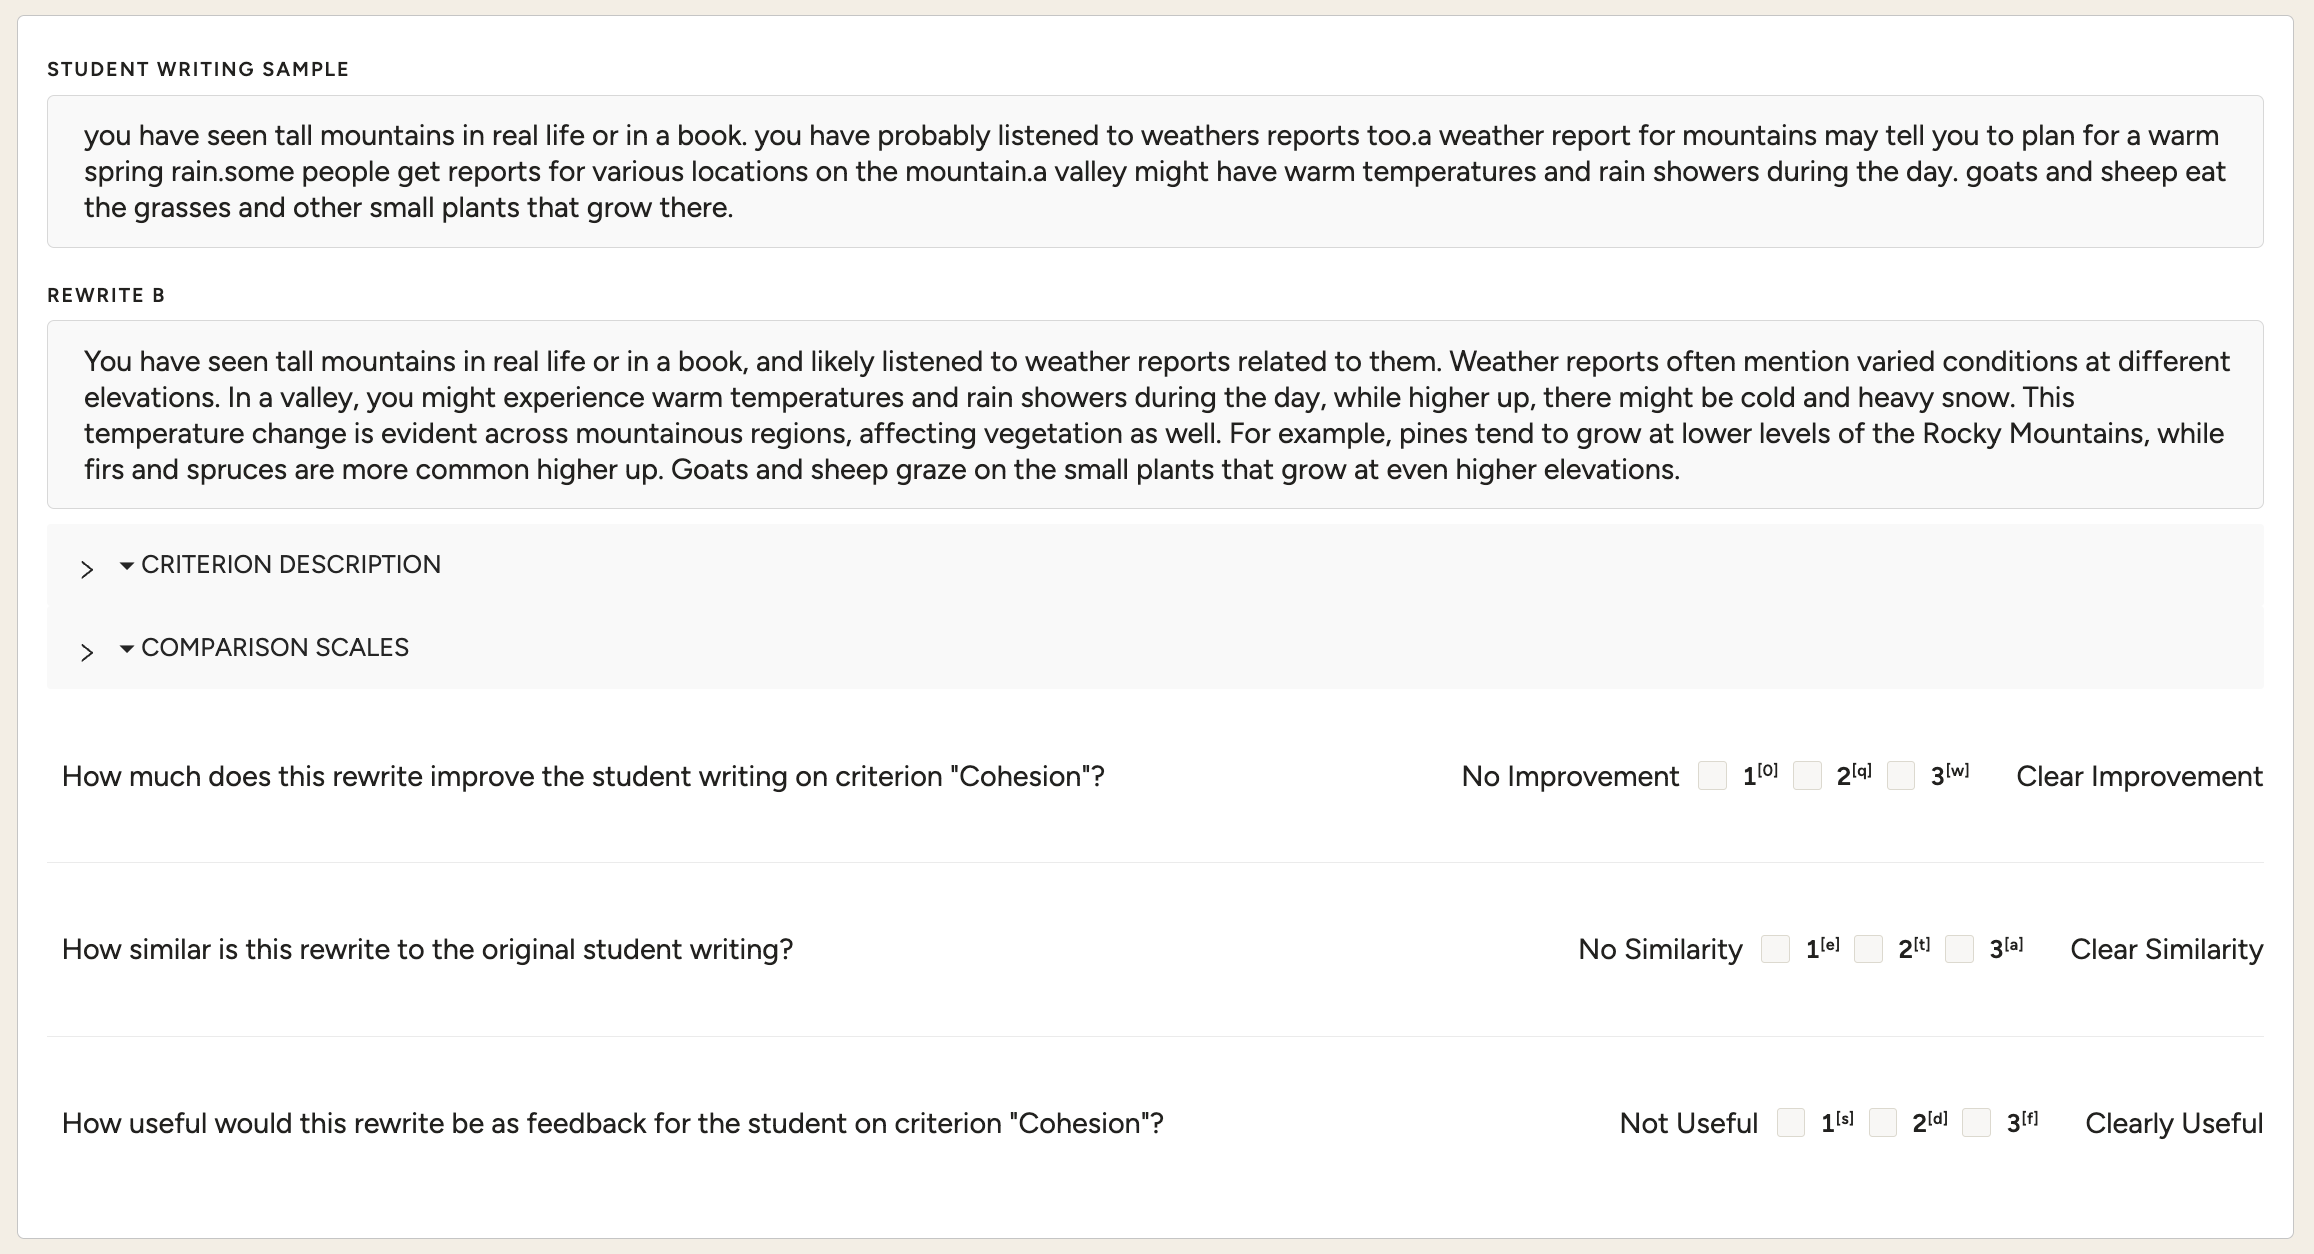
\includegraphics[width=1\linewidth]{label_interface_1.png}
    \caption{Teacher evaluation interface per-rewrite questions (Q1--Q3) for rewrites A and B.}
    \label{fig:label_interface_1}
\end{figure*}

\begin{figure*}[h]
    \centering
    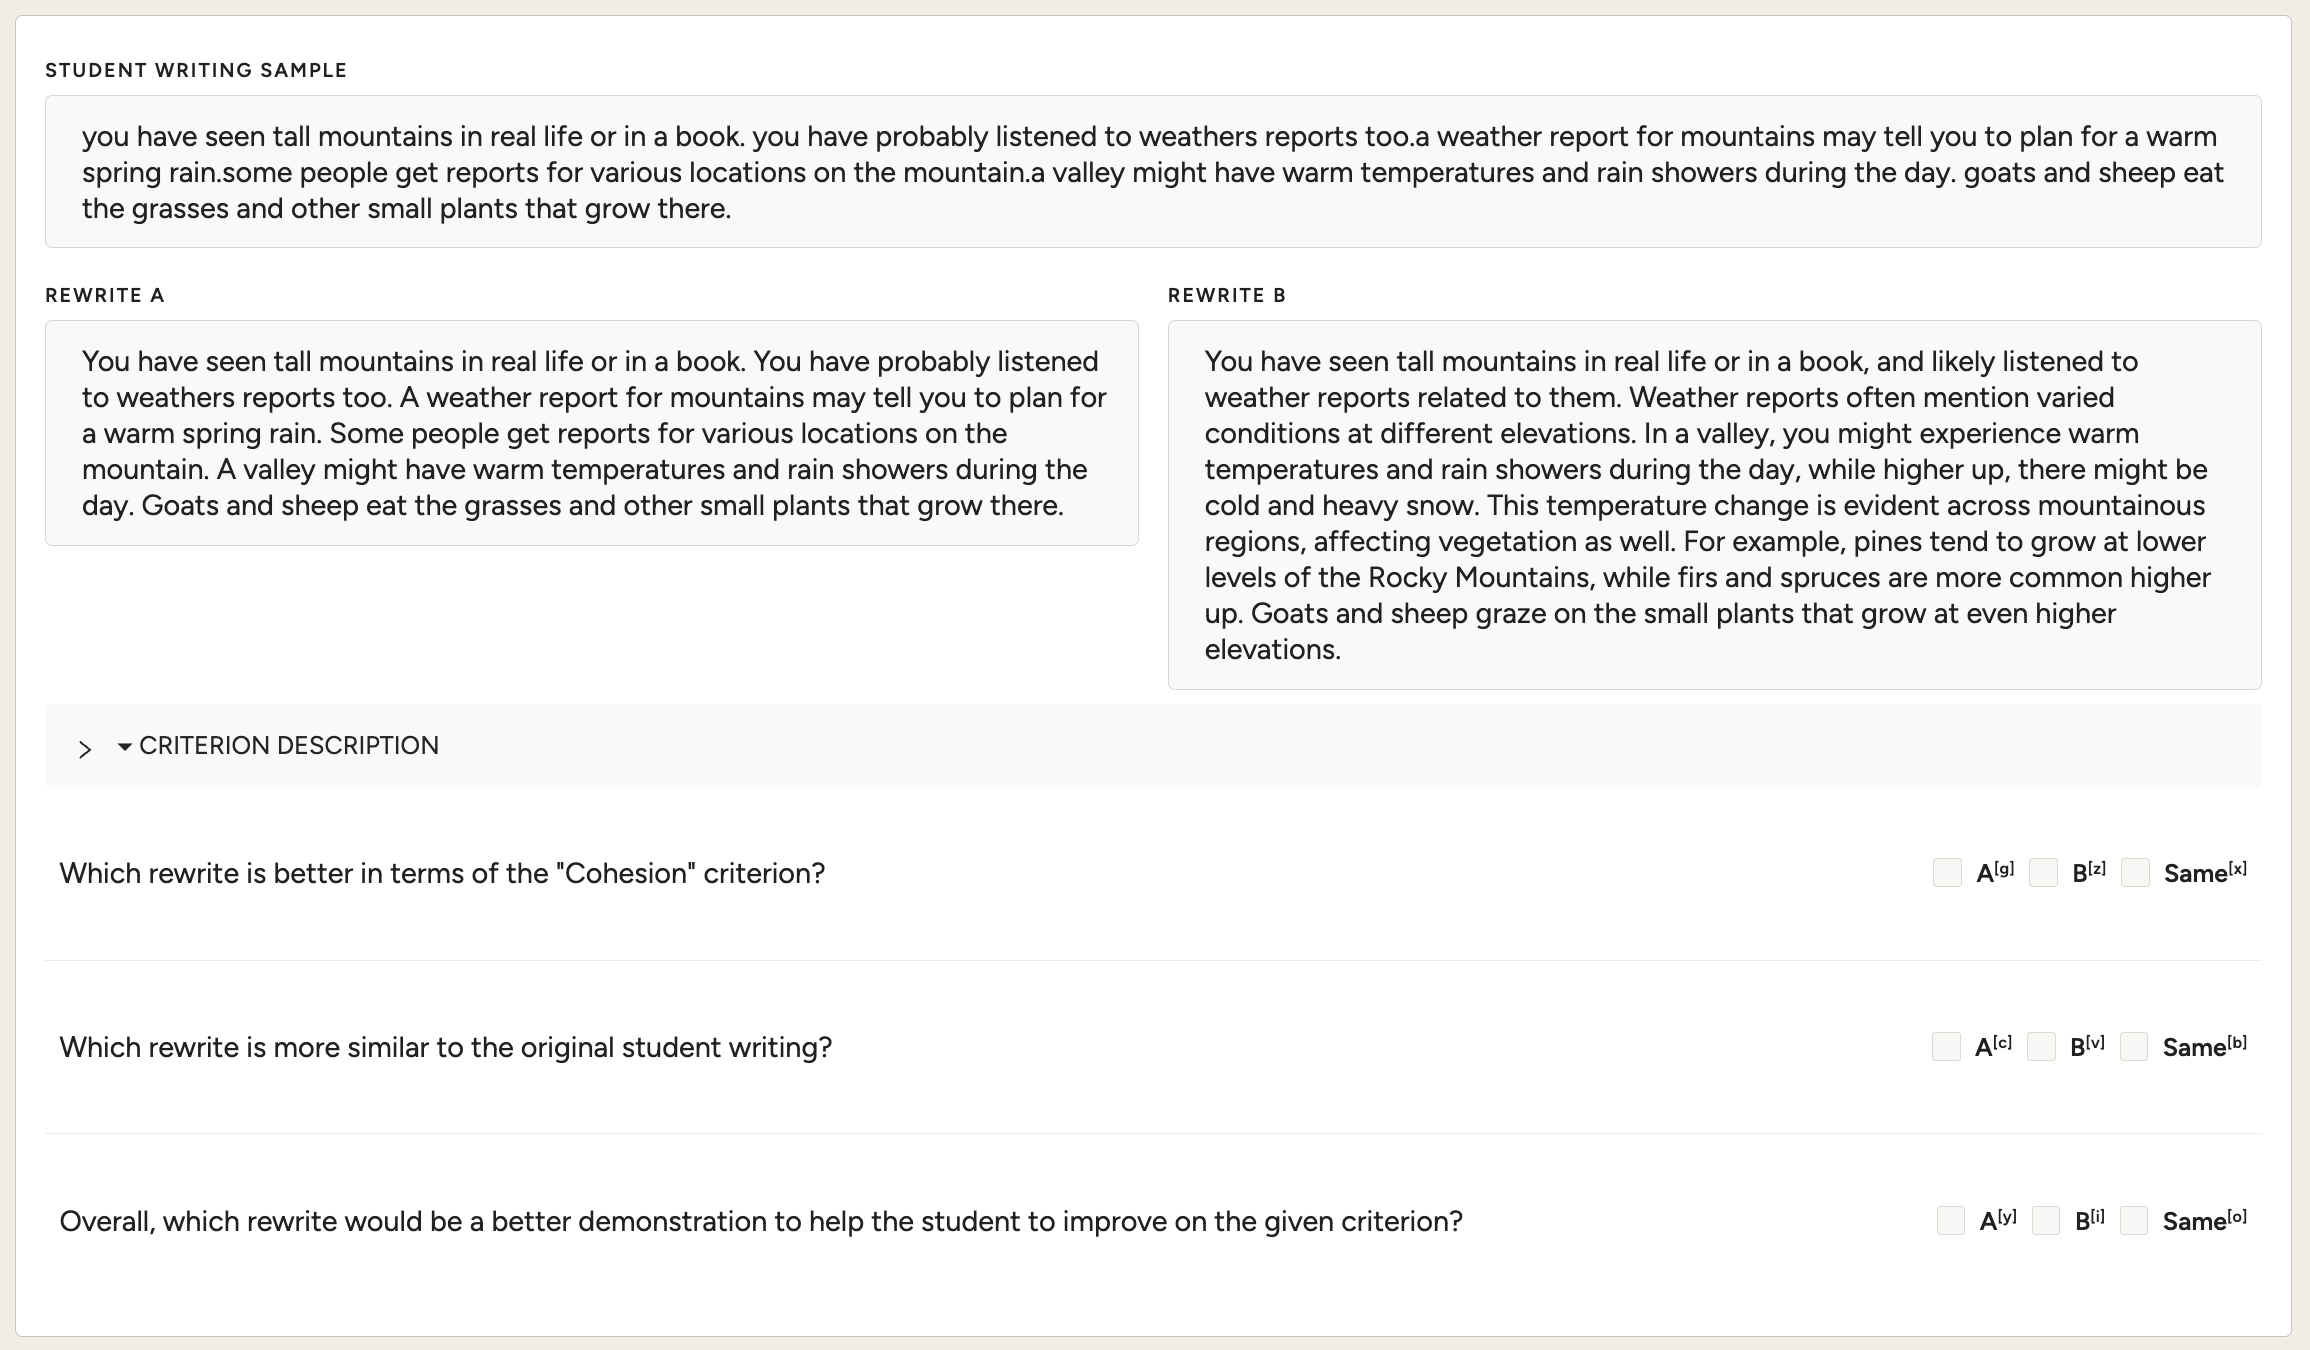
\includegraphics[width=1\linewidth]{label_interface_2.png}
    \caption{Teacher evaluation interface pairwise comparison questions (Q4--Q6).}
    \label{fig:label_interface_2}
\end{figure*}

%% =====================================================================
%% PROMPT BLOCKS
%% =====================================================================

\begin{figure*}
\begin{promptbox}{Example 1: ``Language'' Counterfactual Instruction Prompt}
Your task is to summarize a passage in a way which would receive a score following a set criteria.

You will be given the rubric, the desired scores for each part of the rubric, a passage to summarize, and a reference summary which received a different score.
Use this information to write a summary which would correspond to the given scores and while keeping your summary as close to the reference as possible.

\#\#\# Rubric:

\#\#\# Language Beyond Source Text

**Scores:**

- 1: Poor

- 2: Fair

- 3: Good

- 4: Excellent

**Score Descriptions:**

- **1**: Summary shows a very basic understanding of lexical and syntactic structures.

- **2**: Summary shows an understanding of lexical and syntactic structures.

- **3**: Summary shows an appropriate range of lexical and syntactic structures.

- **4**: Summary shows an excellent range of lexical and syntactic structures.

\#\#\# Passage:

\{\{ reading\_passage\_text \}\}

\#\#\# Desired scores:

**Language Beyond Source Text:** \{\{ language\_score \}\}

\#\#\# Reference Summary:

\{\{ original\_student\_summary \}\}

End your response directly after giving the summary

Do not provide explanation, justification, or notes before or after the summary.

Do not preface with "Here is the summary..."

Do not postface the summary with ``Note'':

\#\#\# Summary:
\end{promptbox}
\caption{Example instruction prompt for ``Language'' criterion including reference. This prompt structure is the basis for Gumbel Machine (GM) and Minimal Edit (ME) structures. In-context Learning (ICL) additionally includes examples after the score descriptions (not shown).}
\label{apx:prompt_ref}
\end{figure*}


\begin{figure*}
\begin{promptbox}{Example 2: ``Details'' Counterfactual Instruction - Excluding Reference}
Your task is to summarize a passage in a way which would receive a score following a set criteria.


You will be given the rubric, the desired score, and a passage to summarize. Use this information to write a summary which would correspond to the given score.


\#\#\# Rubric:

\#\#\# Details

**Scores:**

- 1: Poor

- 2: Fair

- 3: Good

- 4: Excellent

**Score Descriptions:**

- **1**: Statements are not related to the passage.

- **2**: Some key information from the passage is included, but important ideas are missing.

- **3**: Most key information from the passage is included, but some ideas may be irrelevant or inaccurate.

- **4**: All key information in the passage is included without irrelevant ideas.


\#\#\# Passage:

\{\{ reading\_passage\_text \}\}

\#\#\# Desired scores:

**Details:** \{\{ details\_score \}\}

End your response directly after giving the summary

Do not provide explanation, justification, or notes before or after the summary.

Do not preface with "Here is the summary..."

Do not postface the summary with ``Note'':

\#\#\# Summary:
\end{promptbox}
\caption{Example instruction prompt for ``Details'' criterion excluding reference.}
\label{fig:exc_prompt}
\end{figure*}


\begin{figure*}
\begin{promptbox}{Example 3: ``Language'' Identify-and-Replace (I\&R) Prompt --- DREsS}
Your task is to write an essay for a given prompt.

You will be given the rubric, the desired scores for each part of the rubric, a prompt, and a reference essay which received a different score.
Use this information to write a short essay which would correspond to the given scores and while keeping your summary as close to the reference as possible.
Your essay should be similar length to the provided reference text.

\#\# Scoring Rubric

**Language Score** (1--5):

- 1: Very basic or incorrect language use; pervasive errors severely hinder understanding.

- 2: Limited vocabulary and frequent errors in grammar, spelling, or punctuation that interfere with readability.

- 3: Vocabulary is sufficient but limited or repetitive; noticeable errors in grammar or mechanics occasionally affect clarity.

- 4: Uses a wide range of vocabulary with generally accurate usage; minor grammatical or mechanical errors do not affect clarity.

- 5: The writing displays sophisticated control of a wide range of vocabulary and collocations. The essay follows grammar and usage rules throughout the essay. Spelling and punctuation are correct throughout the essay.

\#\# Target Essay Prompt

\{\{ prompt \}\}

\#\# Reference Essay

\{\{ gt\_reference \}\}

\#\# Original Scores

**Language Score:** \{\{ original\_language\_score \}\}

\#\# Desired Scores

**Language Score:** \{\{ language\_score \}\}

Follow this step-by-step reasoning process to write your essay.

STEP\_1: Identify phrases, words, sentences in the Reference essay leading to the Original score.

STEP\_2: Propose minimal edits to those phrases, words, sentences so that the revised essay would receive the Desired score.

STEP\_3: Produce the revised essay by applying the STEP\_2 edits to the Reference essay.

Your goal: rewrite the Reference essay with minimal changes so it would receive the Desired score.

IMPORTANT: The task is NOT complete until the FINAL\_JSON block is printed.

You MUST:

1) Output STEP\_1, STEP\_2, STEP\_3 reasoning.

2) THEN output the FINAL\_JSON block.

3) The FINAL\_JSON block must appear EXACTLY ONCE.

4) The FINAL\_JSON block must be the LAST thing in your response.

5) Do NOT stop after STEP\_3.

6) Do NOT omit the FINAL\_JSON block.

Inside the FINAL\_JSON block:

- Output ONLY valid JSON.

- The JSON must contain exactly one key: ``final\_essay''.

- The value must be a single-line string.

- Do not include newline characters inside the string.

- Do not output any additional text after \texttt{<{}<{}<END\_FINAL\_JSON>{}>{}>}.

SENTINELS (exact):

\texttt{<{}<{}<FINAL\_JSON>{}>{}>}

\{ ``final\_essay'': ``...'' \}

\texttt{<{}<{}<END\_FINAL\_JSON>{}>{}>}
\end{promptbox}
\caption{Example Identify-and-Replace (I\&R) prompt for the DREsS ``Language'' criterion.}
\label{fig:ir_prompt}
\end{figure*}


\begin{figure*}
\begin{promptbox}{Scoring Prompt}
Your task is to give a score for a summary of a passage according to the guidelines given in a rubric.

You will be given a summary that a student wrote for a passage.
For context, you will also be given the passage, which was summarized, and a rubric, which outlines how the summary should be scored for the provided criteria.
You will provide the score and a 1--2 sentence justification in JSON format.
\\ \\
\#\#\# General Guidelines

1.) Make sure to read through the Rubric section below before starting.

2.) You can provide an integer score between 1 and 4 inclusive, that is 1, 2, 3, or 4.

Please make sure you read and understand these instructions carefully. Keep this document open while reviewing, and refer to it as needed.
\\ \\
\#\#\# Output Format

Return your answer as a JSON object with the following structure:

\{

  ``justification'': ``<1--2 sentence justification for your choice>'',

  ``score'': <selected\_score>

\}

- Both fields must be included and non-empty strings. Justification should not exceed two sentences; if multiple lines are needed, concatenate into a single line (no embedded newlines or line breaks).

- Only these two fields should be present in the output JSON.

- Order the JSON fields as shown above: ``justification'' first, then ``label''.

- Both the ``justification'' and ``label'' values must always be strings and must be valid JSON values.

- If the input (summary, passage, or rubric) is missing or empty, output the following JSON: \{ ``justification'': ``ERROR: Cannot score as input information is insufficient or missing.'', ``score'': ``undefined'' \}
\\ \\
\#\#\# Rubric

\#\#\# Criterion: Language Beyond Source Text

\#\#\#\# Description

This criteria measures how well the original aspects of the summary show a mastery of the english language in terms of grammar and vocabulary. The aspects of the summary which are not clearly verbatim copies should be assessed for this criteria. The writers of the summary will be in primary school between grades 3 and 12, so sophisticated, adult-level vocabulary and grammar should not be expected.
\#\#\#\# Possible Scores:

- 1: Poor

- 2: Fair

- 3: Good

- 4: Excellent

\#\#\#\# Score Descriptions:

- **1**: Summary shows a very basic understanding of lexical and syntactic structures.

- **2**: Summary shows an understanding of lexical and syntactic structures.

- **3**: Summary shows an appropriate range of lexical and syntactic structures.

- **4**: Summary shows an excellent range of lexical and syntactic structures.

\#\#\# Passage

\{\{ reading\_passage\_text \}\}

\#\#\# Summary

\{\{ countefactual\_summary \}\}

\#\#\# Score
\end{promptbox}
\caption{Example scoring model prompt for ``Language'' criterion.}
\label{fig:score_prompt}
\end{figure*}


%% =====================================================================
%% CRITERION TABLES
%% =====================================================================

\begin{table*}[!h]
\centering
\renewcommand{\arraystretch}{1.4}
\begin{tabular}{|p{3.5cm}|p{10cm}|}
\hline
\textbf{Criterion} & \textbf{Description} \\
\hline
Main Idea &
This criterion measures how well the main idea of the summary relates to the central topic of the passage. In an ideal summary, the two are closely aligned, and a topic sentence appears at the beginning that clearly captures the main idea. \\
\hline
Details &
This criterion measures how thoroughly and precisely the summary covers the key information discussed in the passage. In an ideal summary, all key information is included, with no irrelevant content or inaccurate representation of the ideas in the passage. \\
\hline
Organization &
This criterion measures how well organized and naturally constructed the summary is. In an ideal summary, each sentence flows naturally into the subsequent sentence without an unnatural or abrupt shift in idea or topic. \\
\hline
Wording &
This criterion measures how well the summary reflects original wording from the passage. While some verbatim copying may be unavoidable for accuracy, an ideal summary paraphrases the passage with minimal direct copying. \\
\hline
Language &
This criterion measures how well the original aspects of the summary demonstrate mastery of English grammar and vocabulary. Portions of the summary that are not verbatim copies should be assessed. Writers range from grades 3 to 12; therefore, sophisticated adult-level language is not expected. \\
\hline
\end{tabular}
\caption{Summary Evaluation Criteria Descriptions}
\label{apx:criteria}
\end{table*}

\begin{table*}[h]
\centering
\renewcommand{\arraystretch}{1.4}
\begin{tabular}{|p{3.5cm}|p{2cm}|p{8.5cm}|}
\hline
\textbf{Criterion} & \textbf{Score} & \textbf{Descriptor} \\
\hline
\multirow{4}{=}{Main Idea}
& 1 (Poor) & Main idea is not linked to the central topic. \\
& 2 (Fair) & Main idea is linked to the central topic, but there is no topic sentence to bring ideas together. \\
& 3 (Good) & Main idea is linked to the central topic and includes a topic sentence stating some aspect of the content. \\
& 4 (Excellent) & Main idea is linked to the central topic and includes a topic sentence that clearly states the main idea. \\
\hline
\multirow{4}{=}{Details}
& 1 (Poor) & Statements are not related to the passage. \\
& 2 (Fair) & Some key information from the passage is included, but important ideas are missing. \\
& 3 (Good) & Most key information is included, but some ideas may be irrelevant or inaccurate. \\
& 4 (Excellent) & All key information from the passage is included with no irrelevant ideas. \\
\hline
\multirow{4}{=}{Organization}
& 1 (Poor) & Ideas are randomly presented and do not link to each other. \\
& 2 (Fair) & Some ideas link to each other. \\
& 3 (Good) & Most ideas are logically presented. \\
& 4 (Excellent) & All ideas are logically presented. \\
\hline
\multirow{4}{=}{Wording}
& 1 (Poor) & Summary shows a heavy reliance on verbatim copying of source language. \\
& 2 (Fair) & Summary shows some use of original wording, but includes verbatim or near-copying of source language. \\
& 3 (Good) & Summary shows evidence of appropriate levels of paraphrasing. \\
& 4 (Excellent) & Summary shows substantial evidence of appropriate paraphrasing use. \\
\hline
\multirow{4}{=}{Language}
& 1 (Poor) & Summary shows a very basic understanding of lexical and syntactic structures. \\
& 2 (Fair) & Summary shows an understanding of lexical and syntactic structures. \\
& 3 (Good) & Summary shows an appropriate range of lexical and syntactic structures. \\
& 4 (Excellent) & Summary shows an excellent range of lexical and syntactic structures. \\
\hline
\end{tabular}
\caption{Detailed definitions and rubrics for each criterion in the CLASSE dataset}
\label{apx:rubric}
\end{table*}

\begin{table*}[!h]
\centering
\renewcommand{\arraystretch}{1.4}
\begin{tabular}{|p{3.5cm}|p{10cm}|}
\hline
\textbf{Criterion} & \textbf{Description} \\
\hline
Content &
This criterion measures how well the essay develops and supports its argument with relevant reasoning and examples. An ideal essay presents well-developed ideas that clearly and thoroughly support the argument. \\
\hline
Organization &
This criterion measures how clearly and logically the essay is structured. An ideal essay has a clear, easy-to-follow argument with effective transitions and coherence devices throughout. \\
\hline
Language &
This criterion measures the student's control of vocabulary and grammatical structures in the essay. An ideal essay demonstrates a wide, accurate range of vocabulary and consistently correct grammar, spelling, and punctuation. \\
\hline
\end{tabular}
\caption{Essay Evaluation Criteria Descriptions for the DREsS dataset.}
\label{apx:dress_criteria}
\end{table*}

\begin{table*}[h]
\centering
\renewcommand{\arraystretch}{1.4}
\begin{tabular}{|p{3.5cm}|p{2.4cm}|p{8.1cm}|}
\hline
\textbf{Criterion} & \textbf{Score} & \textbf{Descriptor} \\
\hline
\multirow{5}{=}{Content}
& 1 (Very Poor) & Paragraph lacks relevance to the argument; little to no supporting reasoning or examples. \\
& 2 (Poor) & Minimal development; ideas unclear or loosely related to argument; weak or vague examples. \\
& 3 (Fair) & Addresses the argument but has limited or uneven development; general reasons with insufficient examples. \\
& 4 (Good) & Relevant and mostly well-developed; clear reasons and some effective examples. \\
& 5 (Excellent) & Well-developed and relevant; strong reasons and examples that clearly support the argument. \\
\hline
\multirow{5}{=}{Organization}
& 1 (Very Poor) & No clear structure; disjointed or random ideas; very difficult to follow. \\
& 2 (Poor) & Difficult to follow; poorly sequenced; limited or ineffective transitions; unclear focus. \\
& 3 (Fair) & Apparent but inconsistent organization; loosely connected ideas; unclear focus or transitions. \\
& 4 (Good) & Clear and logical structure; effective transitions and coherence devices; minor lapses in flow or focus. \\
& 5 (Excellent) & Very effectively structured; easy to follow ideas and argument building; effective coherence devices throughout. \\
\hline
\multirow{5}{=}{Language}
& 1 (Very Poor) & Very basic or incorrect language; pervasive errors severely hinder understanding. \\
& 2 (Poor) & Limited vocabulary; frequent grammar, spelling, or punctuation errors affecting readability. \\
& 3 (Fair) & Sufficient but limited vocabulary; noticeable errors occasionally affect clarity. \\
& 4 (Good) & Wide range of vocabulary with generally accurate usage; minor errors do not affect clarity. \\
& 5 (Excellent) & Sophisticated control of wide vocabulary and collocations; correct grammar, spelling, and punctuation throughout. \\
\hline
\end{tabular}
\caption{Detailed definitions and rubrics for each criterion in the DREsS dataset.}
\label{apx:dress_rubric}
\end{table*}

%% =====================================================================
%% TOKEN COUNT FIGURES
%% =====================================================================

\begin{figure*}
    \centering
    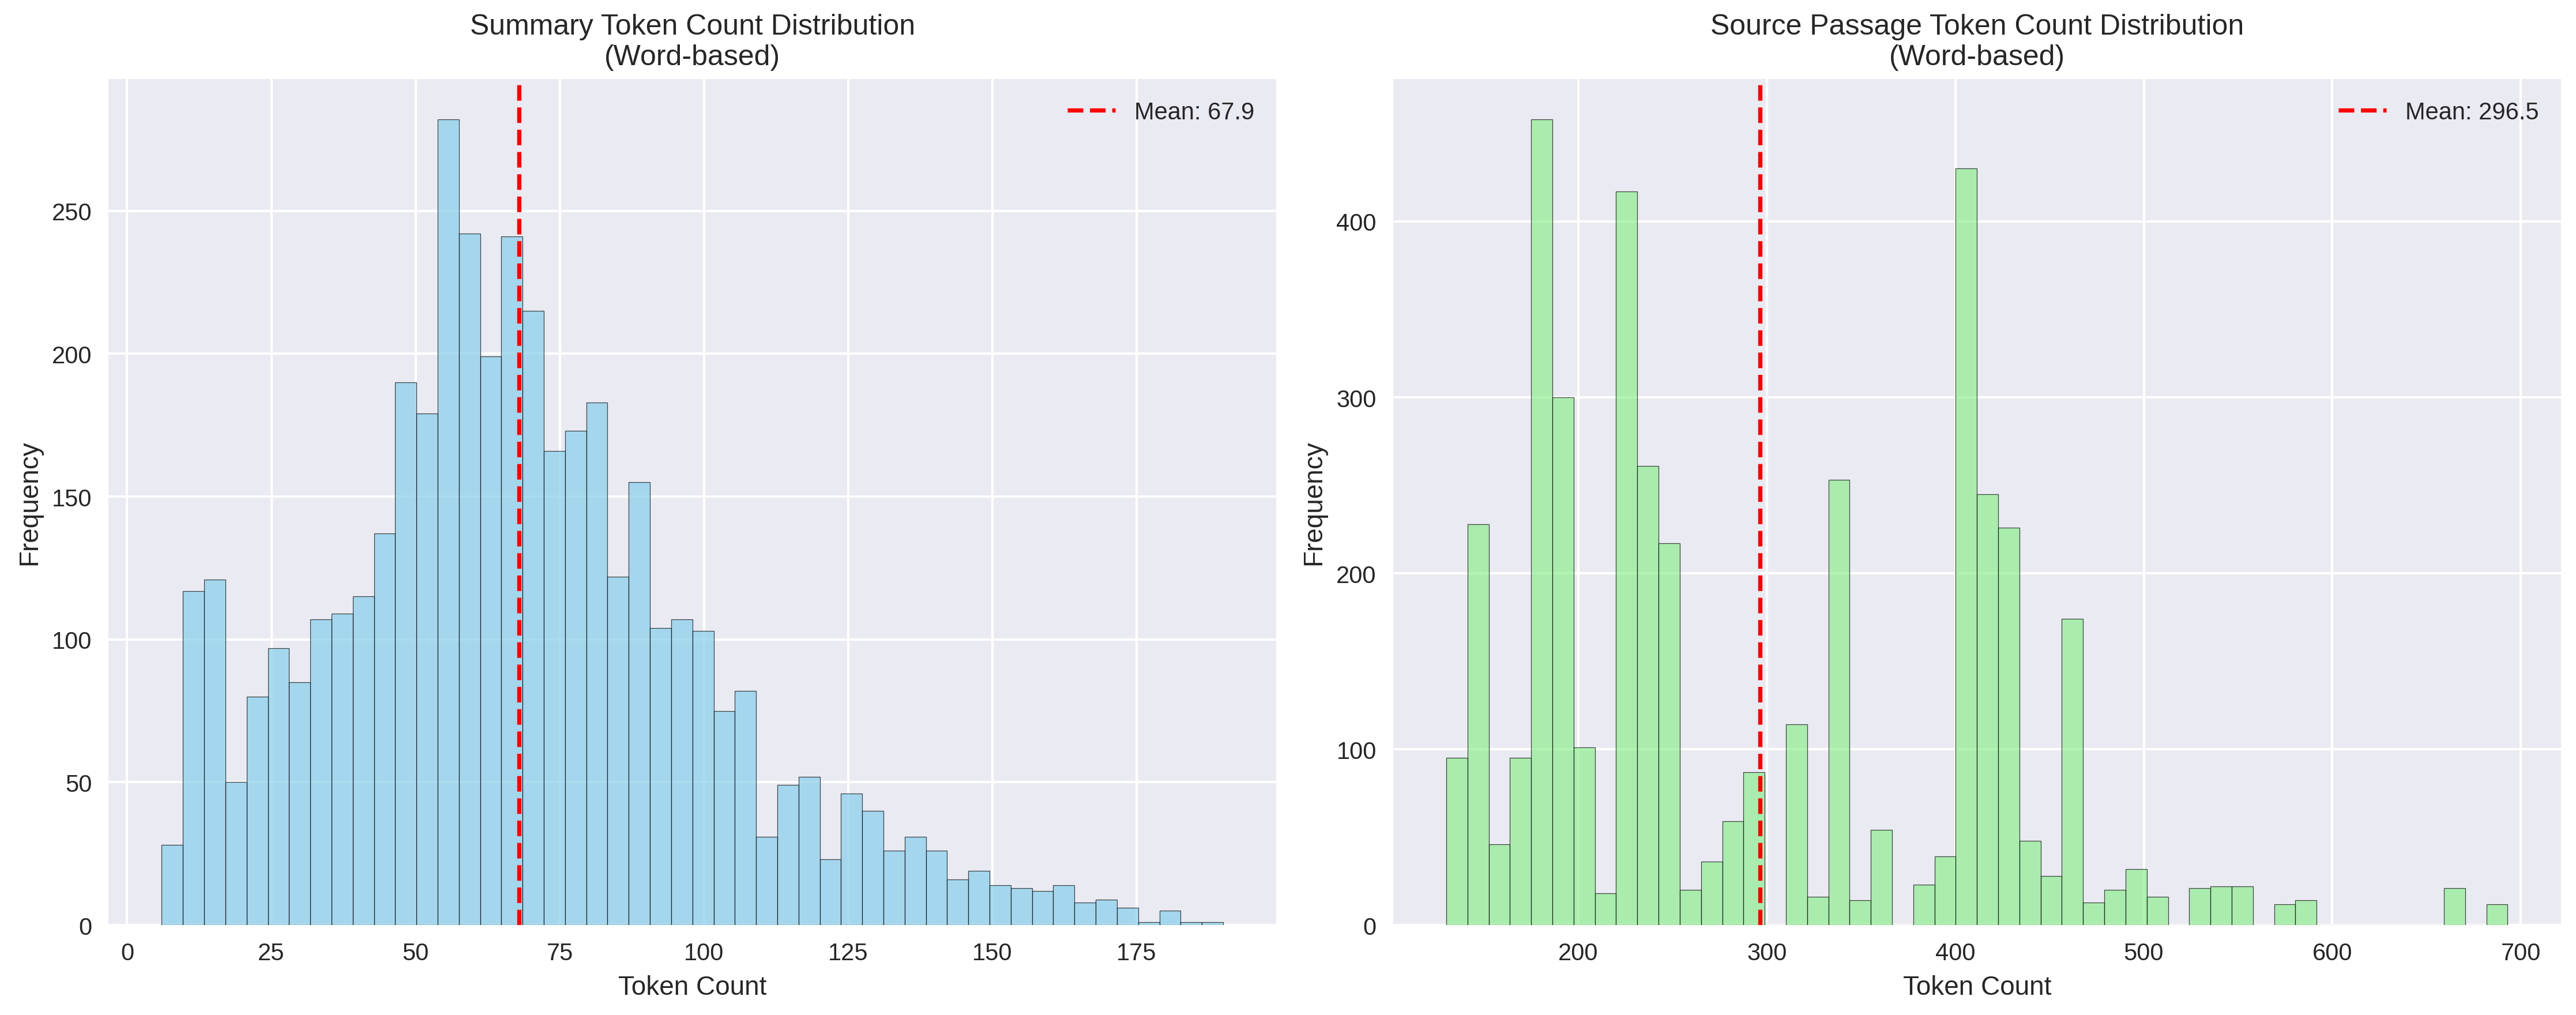
\includegraphics[width=1\linewidth]{token_statistics_visualization_3.jpg}
    \caption{Token count statistics for the summaries and passages in the CLASSE dataset. Summaries are approximately 68 words in length and passages are approximately 297 words.}
    \label{fig:token_counts}
\end{figure*}

\begin{figure*}
    \centering
    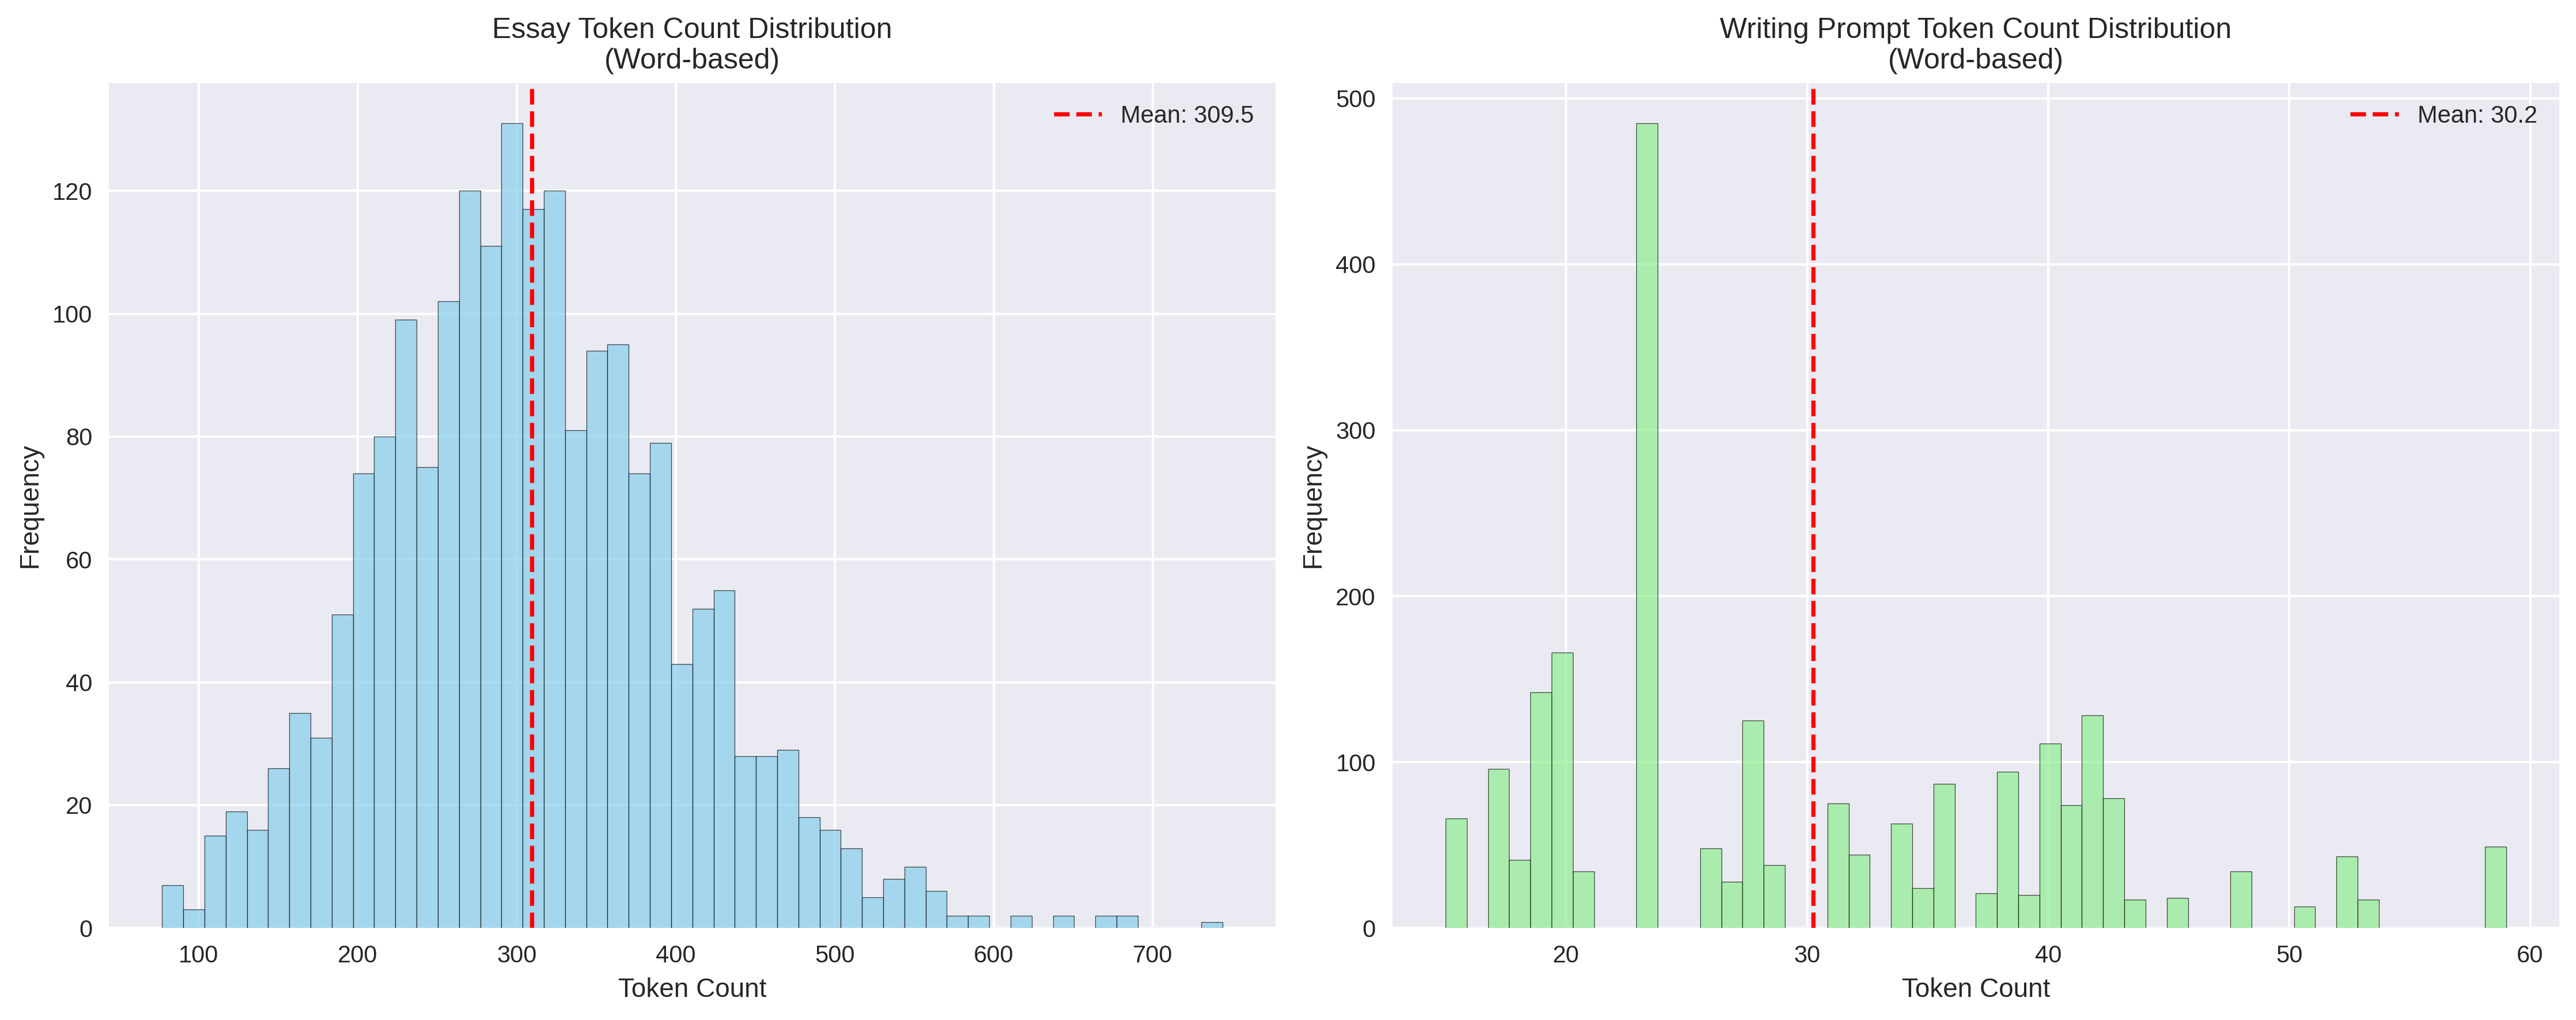
\includegraphics[width=1\linewidth]{dress_token_statistics.png}
    \caption{Token count statistics for the essays and writing prompts in the DREsS dataset. Essays are approximately 310 words in length and writing prompts are approximately 30 words.}
    \label{fig:dress_token_counts}
\end{figure*}

% References cited within the supplementary (aaai2027.sty sets the .bst).
\bibliography{custom}

\end{document}
